\documentclass{scrartcl}
\KOMAoptions{
	%DIV=calc,
	DIV=13,
	fontsize=12pt,
	paper=a4,
}
\linespread{1.2}

\usepackage[utf8]{inputenc} % input-encoding
\usepackage[ngerman]{babel} % deutsche überschriften und silbentrennung
\usepackage{csquotes} % empfohlen bei der verwendung von babel
\usepackage[T1]{fontenc} % mitteleuropäische schriftcodierung mit umlauten etc
\usepackage{lmodern} % lmodern schriften sind schöner als standard

\usepackage{graphicx} % wird benötigt um jpg, pdf, png und tiff bilder einzubinden 
\usepackage{float} % platziert float umgebungen mit H an der stelle an der sie eingebunden werden
\usepackage[section]{placeins} % verhindert, dass Floats hinter dem Befehl \FloatBarrier erscheinen, der mit der option section bei jeder section automatisch gesetzt wird
\usepackage{subcaption}

\usepackage{textcomp} % mehr sonderzeichen
\usepackage{amsmath} % macht mathemathische formeln besser
\usepackage{amsfonts} % macht mathemathische formeln besser
\usepackage{amssymb} % macht mathemathische formeln besser

\usepackage[usenames, dvipsnames]{xcolor}
\definecolor{linkblue}{RGB}{12,77,160}
\definecolor{darkgreen}{RGB}{48, 168, 40}
\definecolor{pflaume}{RGB}{110, 3, 156}
\definecolor{light-gray}{RGB}{220, 220, 220}

\usepackage{tikz}
\usepackage{enumitem}

\usepackage[]{hyperref}  % fügt in der pdf datei u.a. bessere Links ein
\hypersetup{
	%hidelinks,
	colorlinks=true,       % false: boxed links; true: colored links
	linkcolor=linkblue,          % color of internal links (change box color with linkbordercolor)
	citecolor=darkgreen,        % color of links to bibliography
	filecolor=pflaume,         % color of file links
	urlcolor=pflaume,        % color of external links
	pdftitle={Alphaspektroskopie mit einem Halbleiterdetektor},    % title
	pdfauthor={Dennis Spicker},     % author
	pdfsubject={Versuchsanleitung},   % subject of the document
}


\begin{document}
\begin{titlepage}
	\newcommand{\HRule}{\rule{\textwidth}{0.5mm}}
	\begin{center}
	{
\includegraphics[width=0.3\linewidth]{img/GU-Logo-blau-CMYK} \hfill
	
\includegraphics[width=0.3\linewidth]{img/IKF_Logo} \\ }
	\vspace{1cm}
	\HRule
	\vspace{0.4cm}
	{\huge Versuch 12} \\
	\vspace{0.5cm}
	{\huge {\bfseries Alphaspektroskopie}} \\
	\vspace{0.2cm}
	\HRule
	\vfill
	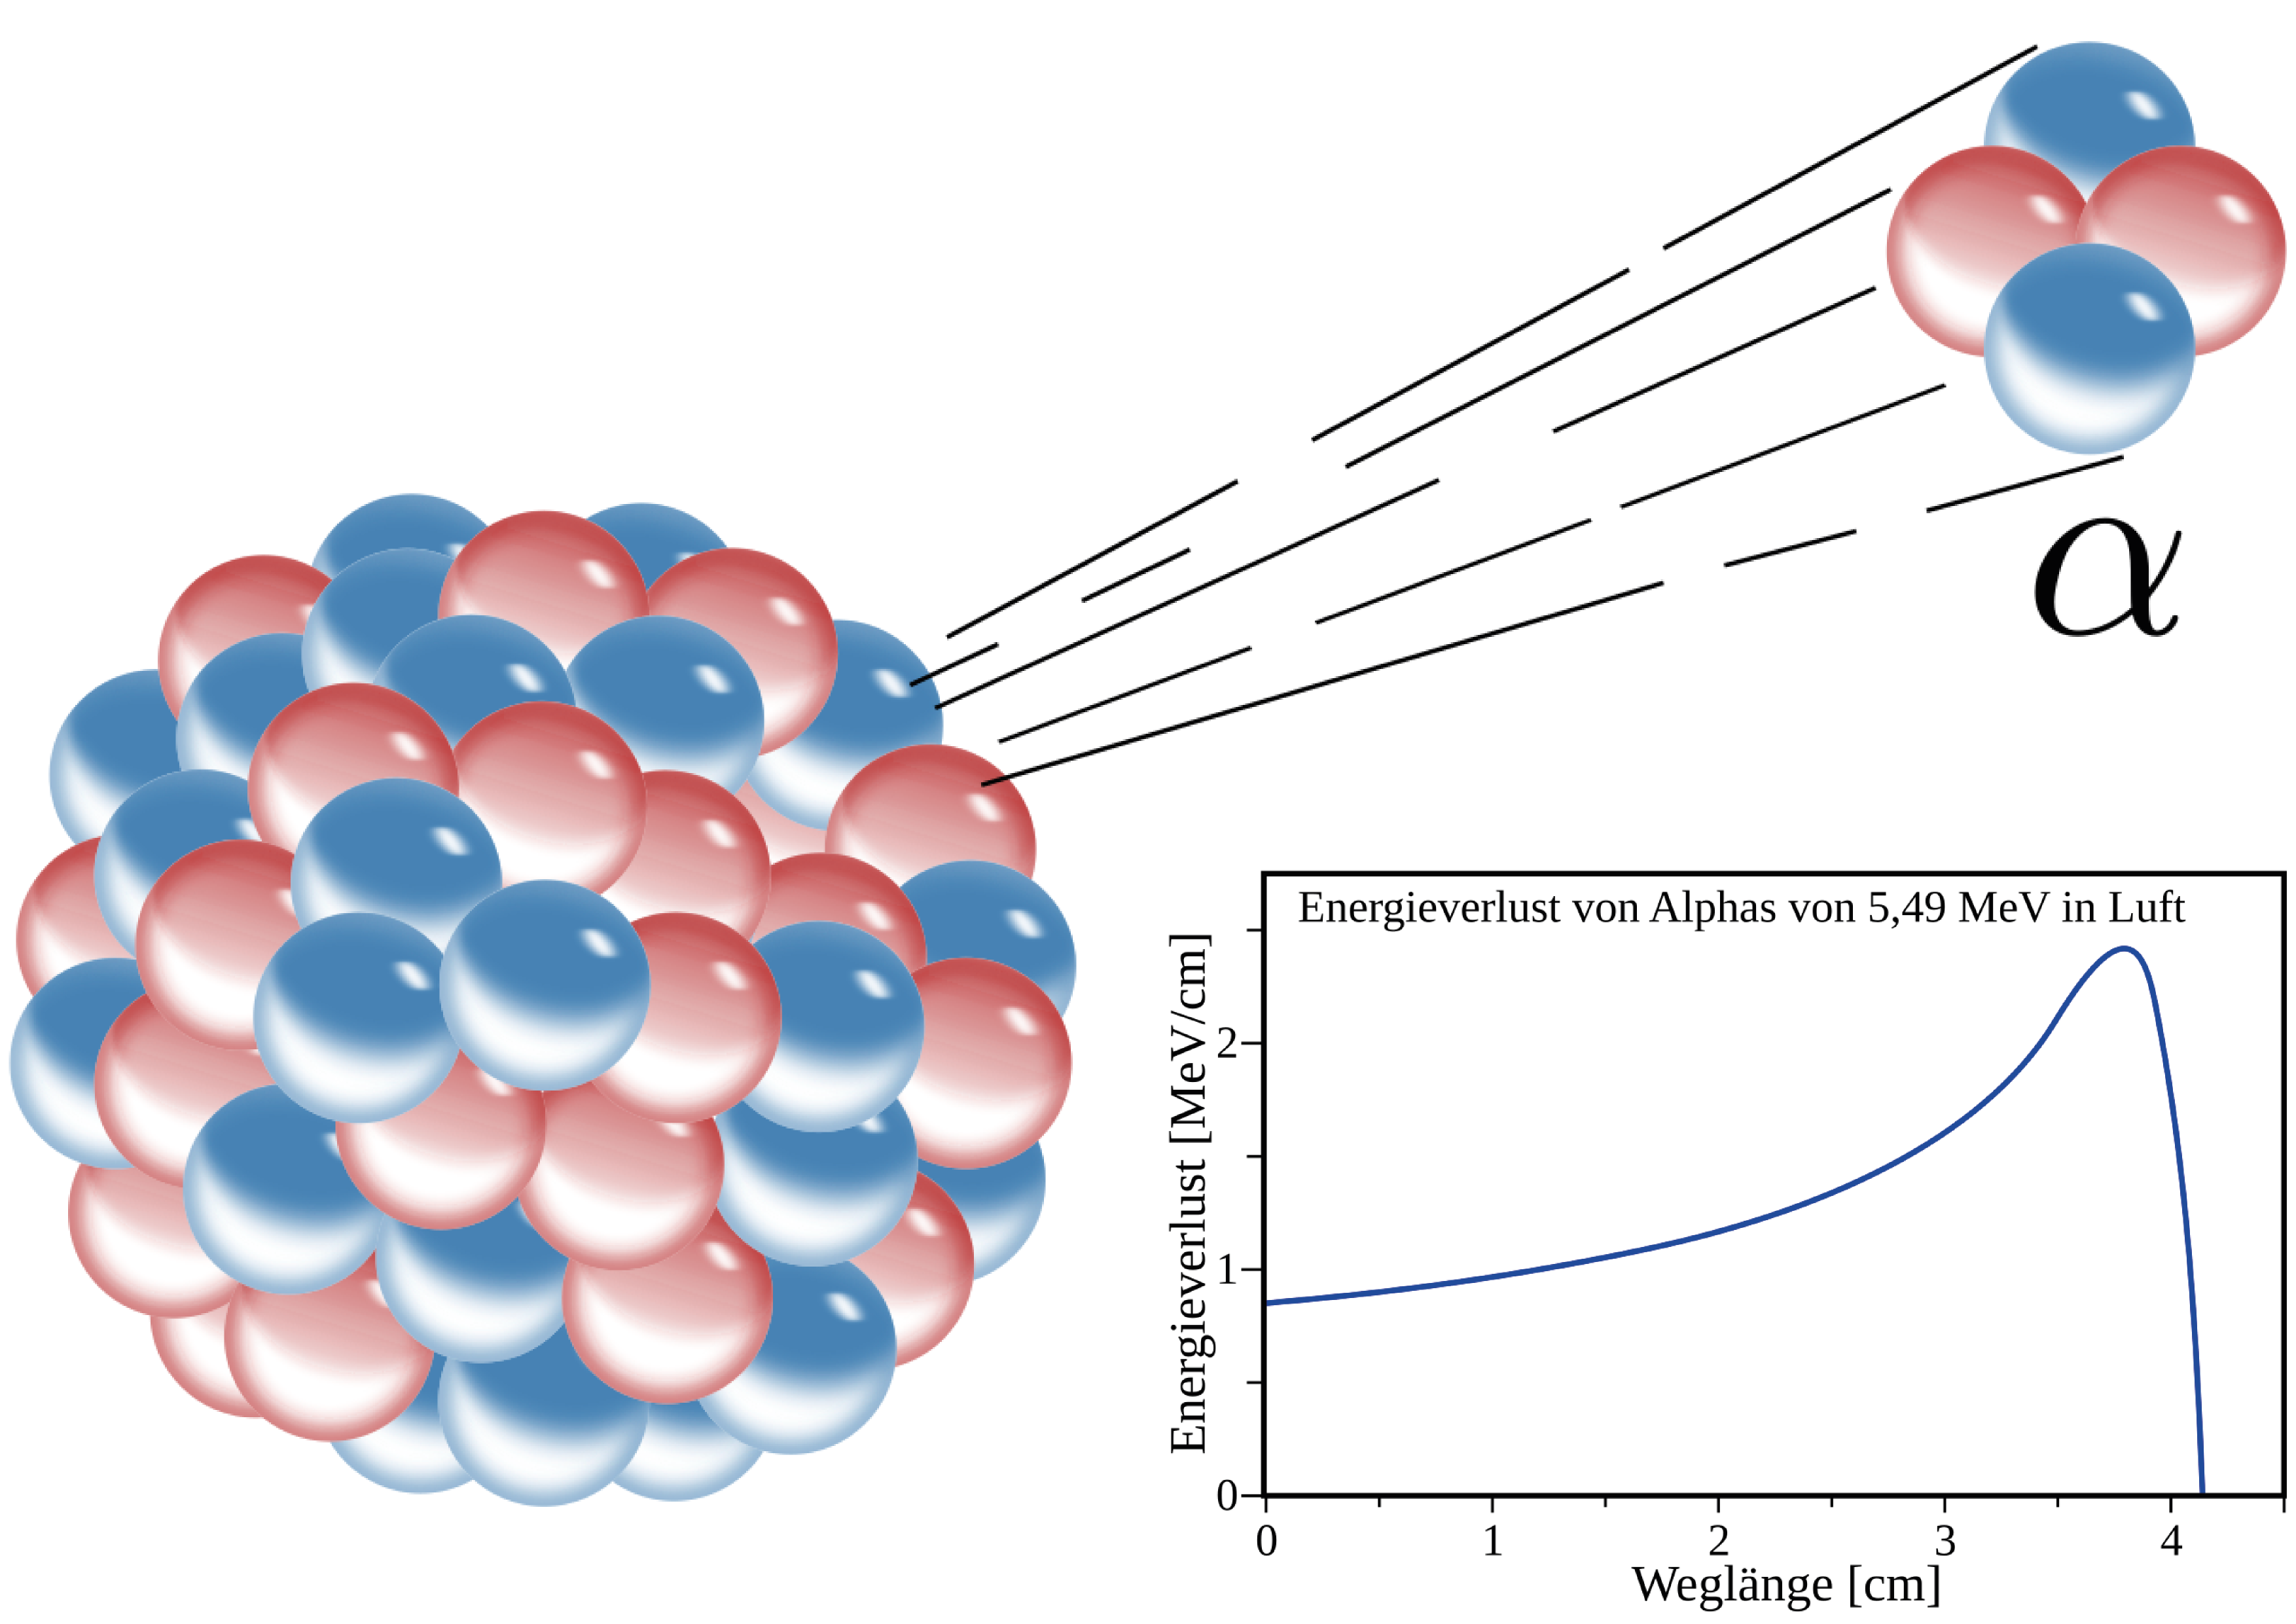
\includegraphics[width=14cm]{img/front_cover.png}
	\vfill
	{\Large\bfseries Fortgeschrittenen Praktikum} \\
	\vspace{0.3cm}
	{\Large am Institut für Kernphysik} \\
	\vspace{1.5cm}
	{\small 
		Dennis Spicker \\
		Juni 2024
	}
	\end{center} 
	\thispagestyle{empty}
	\clearpage
\end{titlepage}
\setcounter{tocdepth}{2}
\tableofcontents
\clearpage





\section{Einführung}
Wenn geladene, schwere Teilchen (z.B. $\alpha$-Teilchen oder schwere Ionen) mit hoher Geschwindigkeit in Materie eindringen, dann geben sie ihre Energie in sehr vielen Zusammenstößen mit den Atomen ab. Dabei gibt es eine Besonderheit: je langsamer sie werden, umso größer ist die abgegebene Energie (sog. Bragg-Kurve). Am GSI Helmholtzzentrum für Schwerionenforschung in Darmstadt wird diese Eigenschaft beispielsweise im Bereich der medizinischen Forschung zur Bestrahlung von Tumoren genutzt.

In diesem Versuch wird Alphastrahlung aus einer Mischquelle mit drei Isotopen mit einem Oberflächensperrschichtzähler gemessen. Ziel ist es, die Strahlung der drei Isotope zu untersuchen. Hierfür werden Energiespektren aufgenommen und daraus die Reichweiten und Bragg-Kurven der Strahlung bestimmt. Dabei werden Sie den Alphazerfall kennenlernen und einen Einblick in die Funktionsweise von Halbleiterdetektoren, die technische Verarbeitung von Signalen und die Auswertung der Daten am Computer erhalten.

Am Versuchstag werden Sie anhand von drei Aufgaben durch den Versuch geführt. Die Aufgaben 1 und 2 befassen sich hauptsächlich mit der Charakterisierung des Versuchsaufbaus und Aufgabe 3 untersucht dann, wie die Alphastrahlung sich im Medium Luft verhält.

\paragraph*{Was Sie wissen müssen, um den Versuch durchzuführen:}
Das nötige Vorwissen für diesen Versuch erstreckt sich auf drei Bereiche: die Theorie des Alphazerfalls, der Energieverlust von geladenen Teilchen in Materie und die Funktionsweise von Halbleiterdetektoren. Die Themen werden in den Unterkapiteln von Abschnitt \ref{sec:theory} kurz vorgestellt.

Für die Versuchsdurchführung ist jedoch noch mehr Wissen nötig, das Sie sich in einer kleinen Literaturrecherche selbst aneignen sollen. Bereiten Sie deshalb bitte die am Ende jedes Unterkapitels angegebenen Themen für den Versuchstag sorgfältig vor. 
Dafür empfehlen sich insbesondere zwei Bücher: "`Teilchendetektoren"' \cite{kolanoski} und "`Teilchen und Kerne"' \cite{povh-rith}, die über die Universitätsbibliothek als PDF-Datei verfügbar sind (Stand Januar 2023).

Nach dem Studium dieser Themen sollten Sie unter anderem die folgenden Fragen beantworten können:
%
\begin{itemize}[itemsep=0pt]
	\item Wie entstehen die Alphateilchen, die in diesem Versuch untersucht werden?
	\item Welche Eigenschaft der Alphateilchen kann mit dem Versuch gemessen werden? 
	\item Hat diese Eigenschaft einen konstanten Wert oder ist sie bei jedem Teilchen anders?
	\item Wie erzeugen die Teilchen ein Signal im Halbleiterdetektor und wie wird das Signal ausgelesen?
	\item Welche Messwerte (Signalwerte) erwarten Sie?
	\item Was sind die hauptsächlichen Quellen von Messungenauigkeiten?
	\item Was ist ein Histogramm?
	\item Welche Informationen stecken in dem Spektrum, das am Computer aufgezeichnet wird?
	\item Wie erhält man aus dem Spektrum die gesuchte Observable (z.B. Energieverlust pro Wegstrecke)?
	\item Was passiert, wenn Luft in der Apparatur ist?
	%Den Bogen Schlagen von Physik Observable zu Messgröße und Messmethode und zurück
\end{itemize}
\newpage
\section{Theoretischer Hintergrund}
\label{sec:theory}
%
\subsection{Alphazerfall}
Alpha"=Teilchen sind identisch mit Helium"=Kernen ( $^4_2$He$^{2+}$ ), sie bestehen also aus jeweils zwei Protonen und Neutronen. Die Bindungsenergie der Nukleonen solcher Alpha"=Teilchen ist stark im Vergleich zu Kernen ähnlicher Größe und beträgt ungefähr 7 MeV pro Nukleon. Die typische kinetische Energie von Alpha"=Teilchen, welche aus natürlichen Zerfällen von radioaktiven Isotopen stammen, liegt im Bereich von $3-8$ MeV \cite{povh-rith}, weitere Eigenschaften können Tabelle \ref{tab:alpha} entnommen werden.
\begin{table}[h]
	\centering
	\begin{tabular}{lc}
		Masse $m_\alpha$    & 3727.3 MeV$/c^{2}$ \\
		Massenzahl A        & 4    \\
		Kernladungszahl Z   & 2    \\
		Bindungsenergie B   & 28.3 MeV \\
	\end{tabular}
	\caption{Eigenschaften der Alpha"=Teilchen.}\label{tab:alpha}
\end{table}

Die Massenzahl des Kerns nimmt beim Alphazerfall um vier Einheiten ab, die Kernladungszahl um zwei Einheiten. Bezeichnet $X$ das Mutter- und $Y$ das Tochternuklid, $\Delta E$  die beim Zerfall frei werdende Energie, und werden wie üblich Massenzahlen $A$ oben und Ordnungszahlen $Z$ unten angeschrieben, gilt für den Alphazerfall allgemein \cite{dewiki:240085809}: 
\begin{equation*}
	^{A}_{Z}X \longrightarrow \ ^{A-4}_{Z-2}Y + \ ^4_2\text{He}^{2+} + \Delta E
\end{equation*}

Beim Alphazerfall wird eine genau definierte Menge an Energie in Form von kinetischer Energie freigesetzt, die der Bindungsenergie des Systems entspricht. Dies ist dank des Phänomens des Massendefekts möglich, bei dem die Masse eines Systems geringer ist als die Summe der Massen seiner Bestandteile. Bei den meisten Alphazerfällen geht der Tochterkern direkt in den Grundzustand über, und die kinetische Energie wird ausschließlich von dem Alphateilchen aufgenommen, wodurch ein monoenergetisches Spektrum entsteht. Es sind jedoch auch Zerfälle in angeregte Zustände des Tochterkerns möglich, bei denen die kinetische Energie zwischen den beiden Teilchen geteilt wird (obwohl das Alpha-Teilchen den größten Teil davon behält), und das Energiespektrum zeigt mehrere monoenergetische Linien, die jeweils einem Zerfall in einen dieser Zustände entsprechen \cite{leo}. Dieses Spektrum ist charakteristisch für das jeweilige Radionuklid und kann daher zu dessen Bestimmung verwendet werden \cite{dewiki:240085809}.

Bevor der Zerfall stattfindet, wird das Alphateilchen einerseits durch die starke Wechselwirkung vom Kern angezogen, aber zugleich aufgrund gleichnamiger Ladungen elektrisch abgestoßen. Die stärkere Kernkraft hat eine kurze, die schwächere elektrostatische Abstoßung eine lange Reichweite. Daher bildet das Potential eine Art Barriere, den Coulombwall (siehe Abb. \ref{fig:coulomb-barriere}). Der Wall ist höher als die für das Alphateilchen verfügbare kinetische Energie. Das Alphateilchen wäre daher nach der klassischen Physik stabil im Kern gebunden; mittels des quantenmechanischen Tunneleffekts kann es ihn jedoch verlassen. Die Wahrscheinlichkeit pro Zeitspanne hierfür kann sehr klein sein. Sie bestimmt die Halbwertszeit des Zerfalls. Der beobachtete Zusammenhang zwischen der Halbwertszeit und der Energie der emittierten Alphateilchen wird durch die Geiger-Nuttall-Regel beschrieben, informieren Sie sich dazu auch über die Gamow-Theorie. \cite{dewiki:240085809}
\begin{figure}[h]
	\centering
	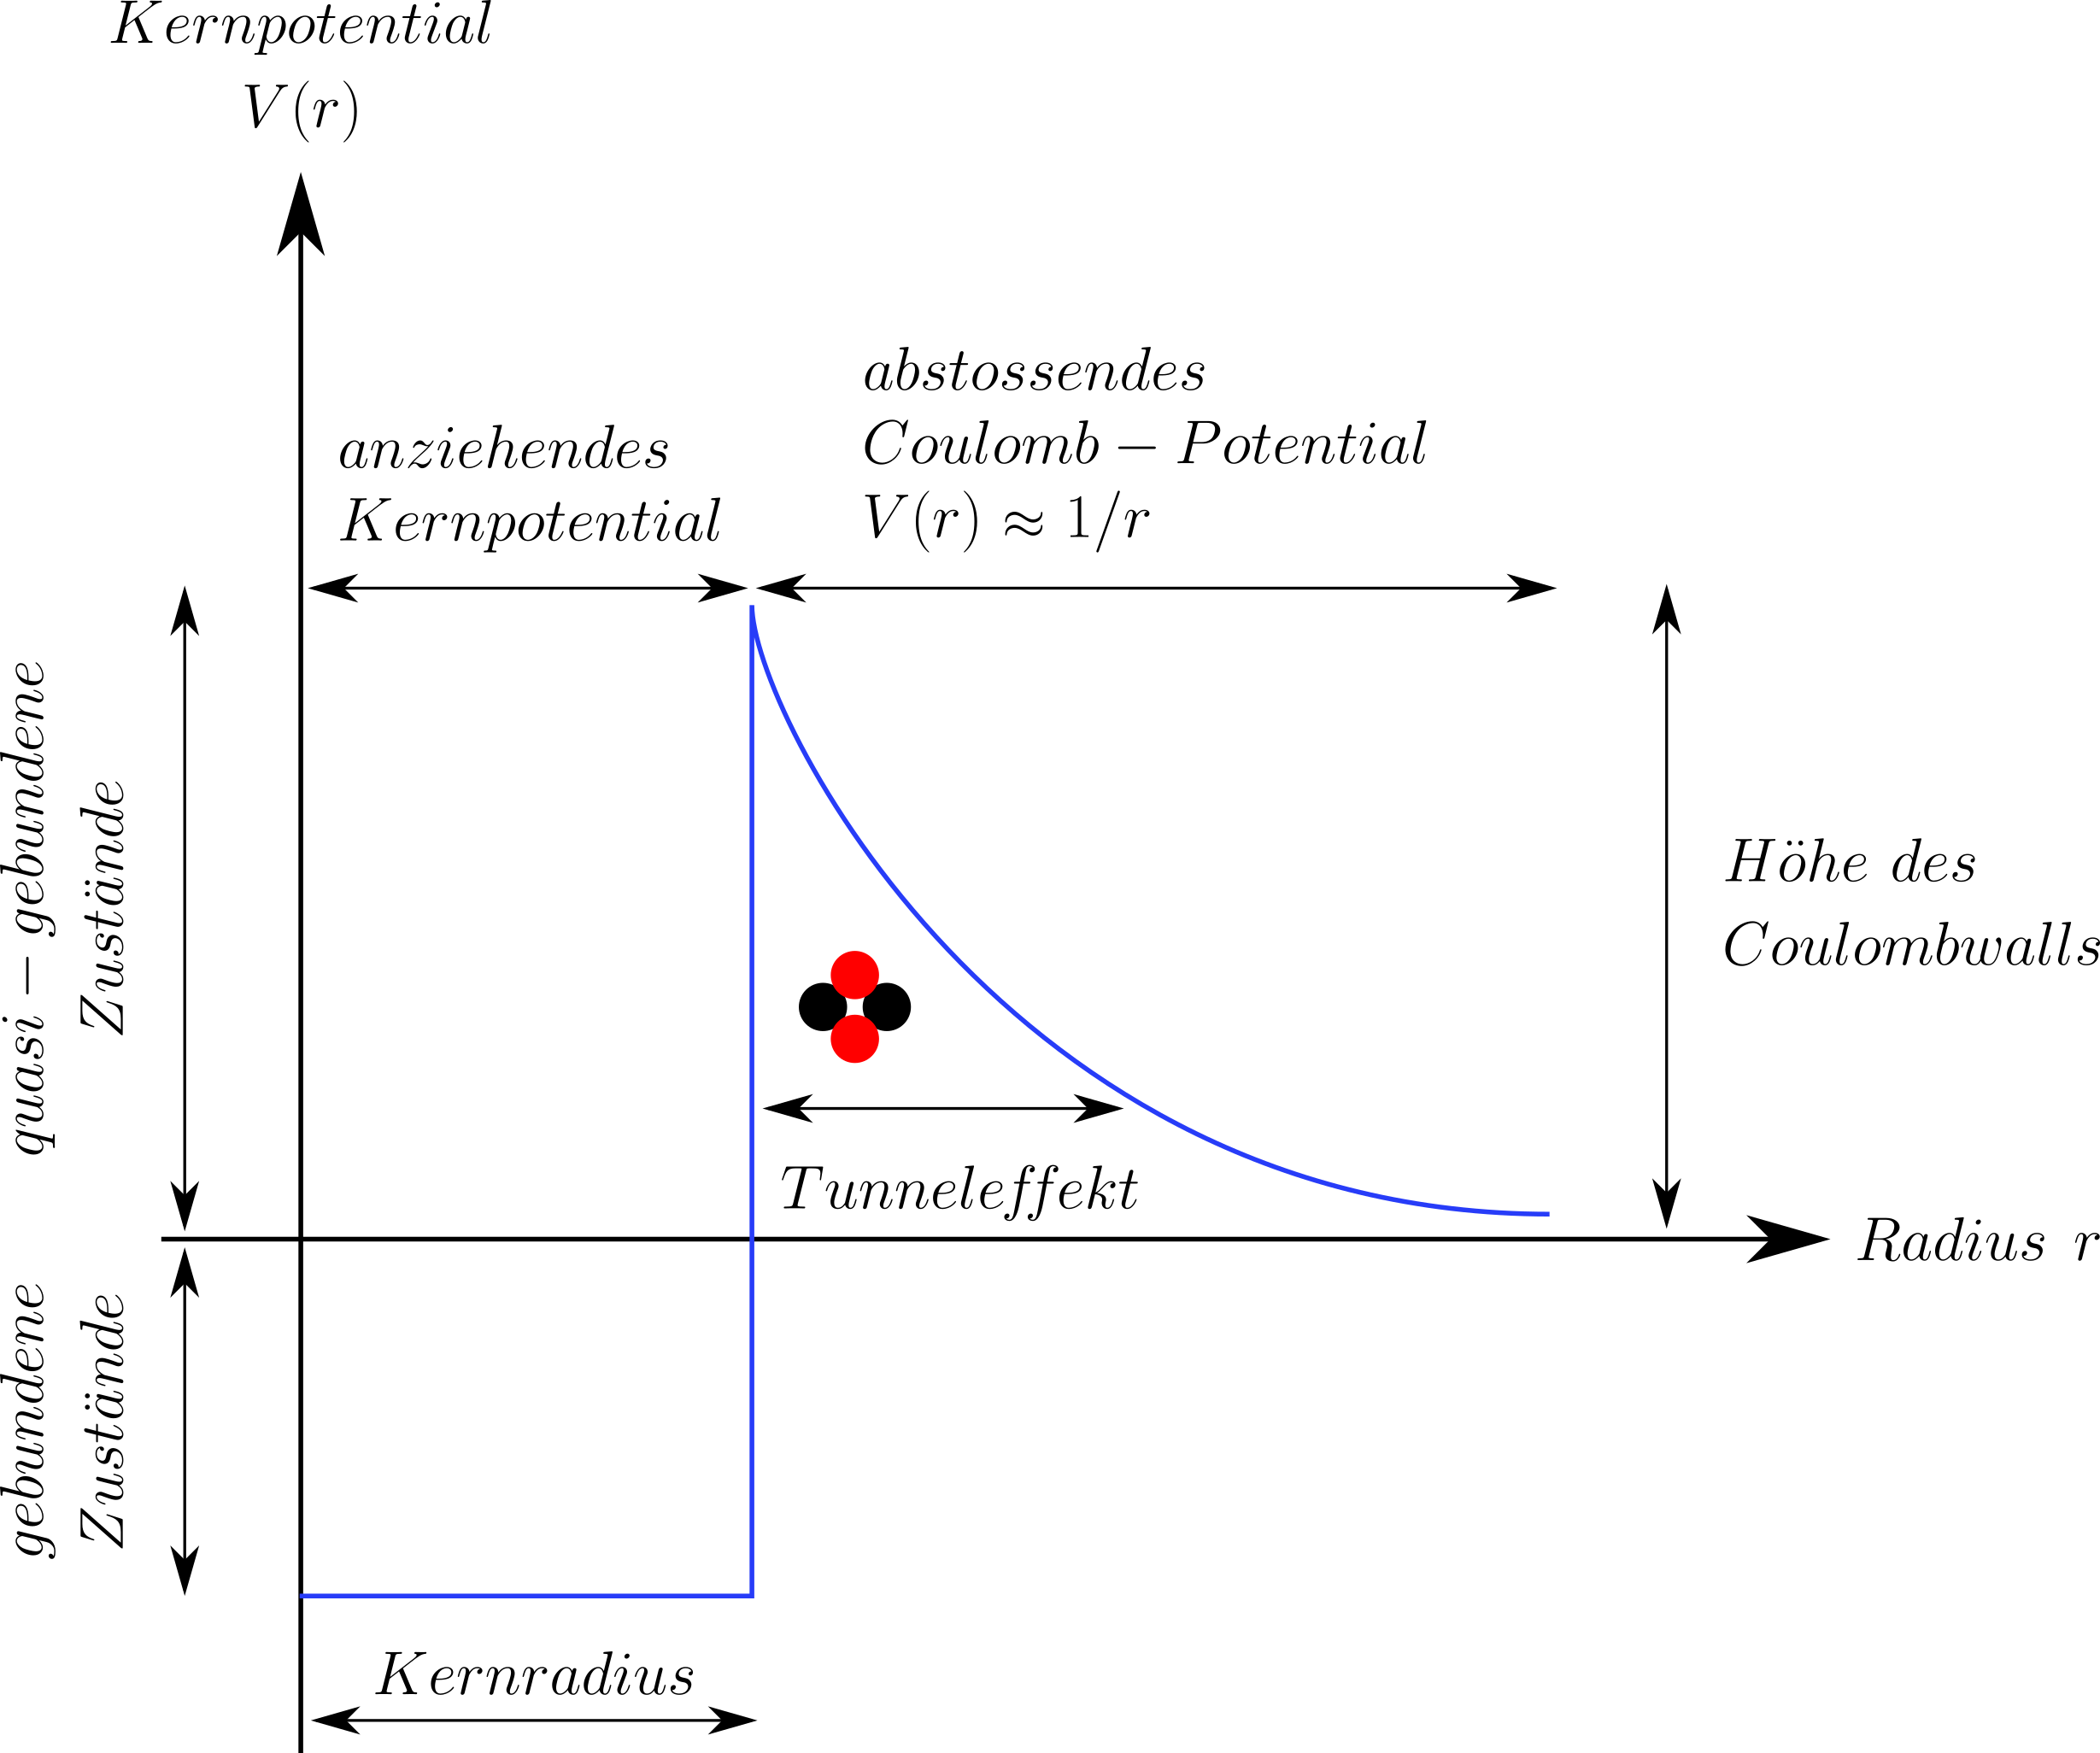
\includegraphics[width=0.6\linewidth]{img/Tunneleffekt_alpha_zerfall.png}
	\caption{Potentielle Energie des Alpha-Teilchens $V(r)$ in Abhängigkeit von seinem Abstand zum Kern $r$. Im negativen Bereich sieht man das durch die starke Kernkraft verursachte Anziehungspotential, im positiven Bereich die Coulombbarriere \cite{img:coulombwall}.}
	\label{fig:coulomb-barriere}
\end{figure}

Die in diesem Versuch untersuchten Alpha"=Teilchen werden von einer Mischquelle, bestehend aus drei verschiedenen Isotopen ($^{239}$Pu, $^{241}$Am, $^{244}$Cm), emittiert. In dem gemessenen Energiespektrum (siehe Abb. \ref{fig:spectrum}) des Alpha"=Strahlers sind neben den Hauptzerfallskanälen auch noch einige Nebenprozesse sichtbar, welche mithilfe der Zerfallstafeln in Abbildung \ref{fig:schemata} identifiziert werden können.

\begin{figure}
	\begin{center}
		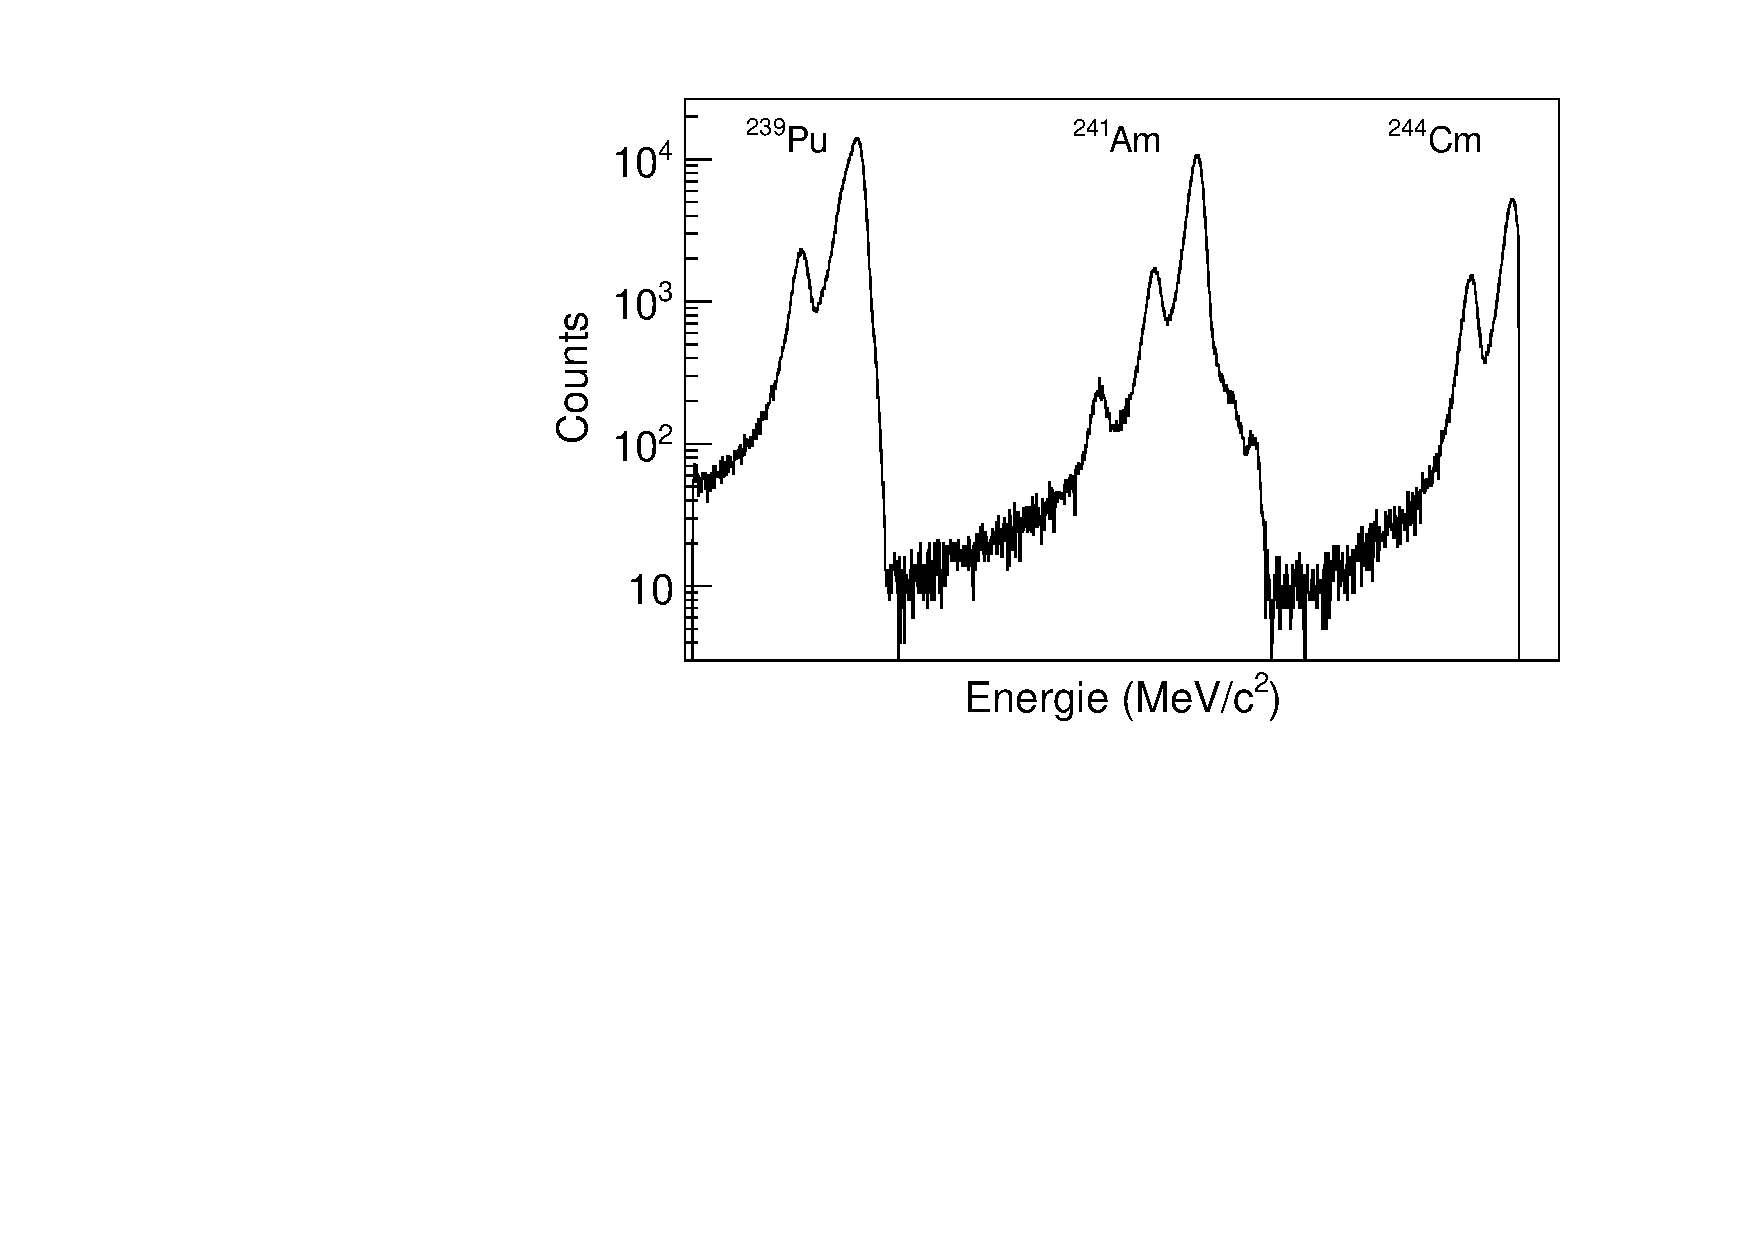
\includegraphics[width=0.9\linewidth]{img/Referenzmessung.pdf}
		\caption{Gemessenes Zerfallsspektrum der verwendeten Mischquelle.}
		\label{fig:spectrum}
	\end{center}
\end{figure}
%
\begin{figure}
	\begin{center}
		\subcaptionbox{Plutonium}{ % I only need the arrows for this one.
%\usepackage{tikz}
%\usetikzlibrary{arrows}
% Place the TikZ picture in a figure environment.
%\begin{figure}
%\centerline{
  % Resize it to 5cm wide.
%\resizebox{horizontal length}{vertical length}{material}
  \resizebox{.3\linewidth}{!}{
    \begin{tikzpicture}[
      scale=0.45,
      level/.style={thick},
      virtual/.style={thick,densely dashed},
      trans/.style={thick,->,shorten >=2pt,shorten <=2pt,>=stealth},
      classical/.style={thin,double,<->,shorten >=4pt,shorten <=4pt,>=stealth}
    ]
    % Draw the energy levels.
    \draw[level] (20em,18em)    -- (40em,18em) node[midway,above] {$^{239}$Pu ($24\cdot10^3$a)};
    \draw[level] (2em,-16em)  -- (21em,-16em) node[midway,above] {$^{235}$U ($7\cdot10^8$a)};
    % Draw the virtual levels.
    \draw[virtual] (4em, 2em)  -- (19em, 2em)  node[midway,above] {5105.8 keV};
    \draw[virtual] (4em,-4em)  -- (19em, -4em)  node[midway,above] {5144.3 keV};
    \draw[virtual] (4em,-10em) -- (19em, -10em) node[midway,above] {5156.59 keV};
    % Draw the transitions.
    \draw[trans] (28em, 18em) -- node[sloped,fill=white] {$11.94\%$} (19em, 2em);
    \draw[trans] (32em, 18em) -- node[sloped,fill=white] {$17.11\%$} (19em, -4em);
    \draw[trans] (36em,18em) -- node[sloped,fill=white] {$70.77\%$} (19em,-10em);
    %    \draw[classical] (4.5cm,-8em) -- (1.5cm,-5em) node[midway,below] {\Ga{}};
    \end{tikzpicture}
  }
%}
%\caption{Zerfallschema}
%\end{figure}


%  \begin{comment}
%  http://www.nndc.bnl.gov/nudat2/decaysearchdirect.jsp?nuc=Pu239&unc=nds
%  
%  Author: E. BROWNE   Citation:Nuclear Data Sheets 98, 665 (2003)
%  
%  Half-Life: 24110 a
%  
%  Alphas:
%  
%  Energy (keV)	Intensity (%)	Dose ( MeV/Bq-s )
%  ...
%  ...
%    4529.6	     3.19E-6 % 3 	  1.445E-7 14 
%    4534	     2.84E-6 % 5 	  1.288E-7 23 
%    4559	     1.2E-5 % 5 	  5.5E-7 23 
%    4632 3 	     7.0E-4 % 20 	  3.2E-5 9 
%    4655	     2.8E-6 % 6 	  1.3E-7 3 
%    4691 3 	     5.0E-4 % 20 	  2.3E-5 9 
%    4718.5	     4.00E-5 % 10 	  1.89E-6 5 
%    4736 3 	     0.0051 % 8 	  2.4E-4 4 
%    4749 5 	     6.0E-4 % 6 	  2.8E-5 3 
%    4769 5 	     0.0015 % 6 	  7E-5 3 
%    4795 4 	     0.0012 % 6 	  6E-5 3 
%    4824	     2.30E-5 % 20 	  1.11E-6 10 
%    4828 3 	     0.0024 % 7 	  1.2E-4 3 
%    4866 5  ?	     0.0019 % 7 	  9E-5 3 
%    4871 5 	     7E-4 % 3 	  3.4E-5 15 
%    4912 5 	     0.0024 % 9 	  1.2E-4 4 
%    4934 3 	     0.0060 % 10 	  3.0E-4 5 
%    4960 5 	     0.0070 % 10 	  3.5E-4 5 
%    4987 3 	     0.0130 % 20 	  6.5E-4 10 
%    5006 5 	     0.0170 % 20 	  8.5E-4 10 
%    5028 3 	     0.009 % 3 	  4.5E-4 15 
%    5054 5 	     0.047 % 13 	  0.0024 7 
%    5076 5 	     0.078 % 8 	  0.0040 4 
%  *  5105.5 8 	    11.94 % 7 	  0.610 4 
%    5111 ?	     0.010 % 10 	  5E-4 5 
%  *  5144.3 8 	    17.11 % 14 	  0.880 7 
%  *  5156.59 14 	    70.77 % 14 	  3.649 7 
%    5156.7	     0.030 % 3 	  0.00155 15 
%  \end{comment}
 }
		\subcaptionbox{Americium}{ % I only need the arrows for this one.
%\usepackage{tikz}
%\usetikzlibrary{arrows}
% Place the TikZ picture in a figure environment.
%\begin{figure}
%\centerline{

% Resize it to 5cm wide.
  \resizebox{.3\linewidth}{!}{
  \begin{tikzpicture}[
      scale=0.45,
      level/.style={thick},
      virtual/.style={thick,densely dashed},
      trans/.style={thick,->,shorten >=2pt,shorten <=2pt,>=stealth},
      classical/.style={thin,double,<->,shorten >=4pt,shorten <=4pt,>=stealth}
    ]
    % Draw the energy levels.
    \draw[level] (20em,18em)    -- (40em,18em) node[midway,above] {$^{241}$Am (432.6a)};
    \draw[level] (2em,-16em)  -- (21em,-16em) node[midway,above] {$^{237}$Np ($2.1\cdot10^6$a)};
    % Draw the virtual levels.
    \draw[virtual] (4em,9em)  -- (19em,9em)  node[midway,above] {5388.0 keV};
    \draw[virtual] (4em,4em)  -- (19em,4em)  node[midway,above] {5442.8 keV};
    \draw[virtual] (4em,-1em) -- (19em,-1em) node[midway,above] {5485.56 keV};
    \draw[virtual] (4em,-6em) -- (19em,-6em) node[midway,above] {5511.5 keV};
    \draw[virtual] (4em,-11em) -- (19em,-11em) node[midway,above] {5544.5 keV};
    % Draw the transitions.
    \draw[trans] (26em, 18em) -- node[sloped,fill=white] {$1.66\%$}  (19em, 9em);
    \draw[trans] (29em, 18em) -- node[sloped,fill=white] {$13.1\%$} (19em, 4em);
    \draw[trans] (32em,18em) -- node[sloped,fill=white] {$84.8\%$}  (19em,-1em);
    \draw[trans] (35em,18em) -- node[sloped,fill=white] {$0.225\%$}  (19em,-6em);
    \draw[trans] (38em,18em) -- node[sloped,fill=white] {$0.37\%$}  (19em,-11em);
    %    \draw[classical] (4.5em,-8em) -- (1.5em,-5em) node[midway,below] {\Ga{}};
    \end{tikzpicture}
  }
%}
%\caption{Zerfallsschema Alphazerfalll von $^{241}$Am.}
%\end{figure}

%  http://www.nndc.bnl.gov/nudat2/decaysearchdirect.jsp?nuc=241AM&unc=nds
%  Author: M. S. Basunia   Citation:Nuclear Data Sheets 107, 3323 (2006)
%  Half-Life: 432.6
%  Alphas:
%  Energy (keV)   Intensity (%)   Dose ( MeV/Bq-s )
%    4758         5E-6 % 5    2.4E-7 24 
%    4800         8.6E-5 %   4.128E-6
%    4834         7E-4 %   3.384E-5
%    5004         1E-4 %   5.004E-6
%    5068         1.4E-4 %   7.0952E-6
%    5089         4.0E-4 % 4    2.04E-5 20 
%    5096         4.0E-4 % 4    2.04E-5 20 
%    5114         4E-4 %   2.0456E-5
%    5137         3.2E-4 %   1.644E-5
%    5155         7E-4 %   3.609E-5
%    5178         3E-4 %   1.553E-5
%    5182         9E-4 %   4.664E-5
%    5192         6E-4 %   3.115E-5
%    5217         1.0E-5 % 10    5E-7 5 
%    5223         0.0013 %   6.79E-5
%    5244         0.0024 %   1.259E-4
%    5279         5E-4 %   2.64E-5
%    5322         0.015 % 5    8E-4 3 
%  * 5388         1.660 % 20    0.0894 11 
%    5416.5       0.0100 % 10    5.4E-4 5 
%  * 5442.80 13   13.1 % 3    0.713 16 
%    5469         0.020 % 20    0.0011 11 
%  * 5485.56 12   84.8 % 5    4.65 3 
%  * 5511.5       0.225 % 5    0.0124 3 
%  * 5544.5  16   0.37 % 3    0.0205 17
 }
		\subcaptionbox{Curium}{ % I only need the arrows for this one.
%\usepackage{tikz}
%\usetikzlibrary{arrows}
% Place the TikZ picture in a figure environment.
%\begin{figure}
%\centerline{
  % Resize it to 5cm wide.
  \resizebox{.3\linewidth}{!}{
    \begin{tikzpicture}[
      scale=0.45,
      level/.style={thick},
      virtual/.style={thick,densely dashed},
      trans/.style={thick,->,shorten >=2pt,shorten <=2pt,>=stealth},
      classical/.style={thin,double,<->,shorten >=4pt,shorten <=4pt,>=stealth}
    ]
    % Draw the energy levels.
    \draw[level] (20em,18em)   -- (40em,18em) node[midway,above] {$^{244}$Cm ($18.11$a)};
    \draw[level] (2em,-16em)  -- (21em,-16em) node[midway,above] {$^{240}$Pu ($6561$a)};
    % Draw the virtual levels.
    \draw[virtual] (4em,-6em)  -- (19em,-6em)  node[midway,above] {5762.46 keV};
    \draw[virtual] (4em,-11em)  -- (19em,-11em)  node[midway,above] {5804.77 keV};
    %    \draw[virtual] (0cm,-11em) -- (4cm,-11em) node[midway,above] {5.155 MeV};
    % Draw the transitions.
    \draw[trans] (29em, 18em) -- node[sloped,fill=white] {$23.1\%$} (19em, -6em);
    \draw[trans] (32em, 18em) -- node[sloped,fill=white] {$76.9\%$} (19em, -11em);
    %    \draw[classical] (4.5cm,-8em) -- (1.5cm,-5em) node[midway,below] {\Ga{}};
    \end{tikzpicture}
  }
%}
%\caption{Zerfallsschema}
%\end{figure}


%  Authors: BALRAJ SINGH, E. BROWNE   Citation:Nuclear Data Sheets 109,
%  2439 (2008)
%  
%  http://www.nndc.bnl.gov/nudat2/decaysearchdirect.jsp?nuc=244CM&unc=nds
%  
%  Half-Life: 18.11a
%  
%  Alphas:
%  
%  Energy 
%  (keV)	Intensity 
%  (%)	Dose 
%  ( MeV/Bq-s )
%    4920 3 	     5.0E-5 % 5 	  2.46E-6 25 
%    4960 3 	     1.49E-4 % 16 	  7.4E-6 8 
%    5166.64 7 	     4E-6 % 3 	  2.1E-7 15 
%    5215 3 	     5.6E-5 % 5 	  2.9E-6 3 
%    5315	     4E-5 %	  2.126E-6
%    5513 3 	     0.00352 % 18 	  1.94E-4 10 
%    5664 3 	     0.0204 % 15 	  0.00116 8 
%  *  5762.64 3 	    23.10 % 10 	  1.331 6 
%  *  5804.77 5 	    76.90 % 10 	  4.464 6 
%  

 }
		\caption{Zerfallsschemata der Nuklide des Alphastrahlers. \\Datenquellen: Pu~\cite{NDS2014}, Am~\cite{NDS2006}, Cm~\cite{NDS2008}}
		\label{fig:schemata}
	\end{center}
\end{figure}
%
\paragraph{Themen zur Vorbereitung}
\begin{itemize}
	\item Bindungsenergie von Atomkernen, Massendefekt
	\item Nuklidkarte, Stabilität von Kernen
	\item Abstandsquadratgesetz
	%\item Magische Zahlen (Schalenmodell des Atomkerns).
	%\item Alpha-Zerfall allgemein.
	\item Linienspektrum des Alphazerfalls
	\item Eigenschaften der Nukleonen
	\item Gamow-Theorie des Alphazerfalls, Gamow-Faktor, Lebensdauer, Potenzial des Atomkerns, Tunneleffekt
\end{itemize}
\FloatBarrier
\subsection{Wechselwirkung von geladenen Teilchen in Materie}
% Geiger-Nuttall-Regel
% citation for ionsation potential in air:
% http://onlinelibrary.wiley.com/doi/10.1002/andp.19614630504/abstract;jsessionid=E4B5E16EA9E0D4DAD7454073D3773C23.f02t02
Beim Durchdringen von Materie verlieren Alpha"=Teilchen ihre Energie im Wesentlichen durch Ionisation und Anregung der Atome im Material. Da sie deutlich massiver sind als die Elektronen des Materials ($m_\alpha \approx 8000\ m_{e}$) mit denen sie wechselwirken, passieren sie das Material ohne große Ablenkungen. Der mittlere Energieverlust pro Weglänge wird durch die Bethe"=Bloch"=Formel beschrieben \cite{kolanoski}. Er hängt von den Eigenschaften des Mediums sowie von der Ladung und der Geschwindigkeit des Teilchens ab.
\begin{equation}
	\left\langle - \frac{dE}{dx} \right\rangle = K \frac{Z}{A} \frac{z^2}{\beta^2} \ \left[ \frac{1}{2} \ln \left( \frac{2 m_e c^2 \beta^2 \gamma^2 T_{max}}{I^2} \right) - \beta^2 - \frac{\delta(\beta\gamma)}{2} \right] 
\end{equation}
\begin{itemize}[itemsep=0pt, label=-]
	\item $K=4\pi N_A r_e^2 m_e c^2 = 0.307\ \text{MeV cm}^2 / \text{mol} $ mit $r_e \approx 2.8$ fm;
	\item $z$ Ladungszahl, $\beta = v / c$ Geschwindigkeit des Projektilteilchens;
	\item $Z$ Kernladungszahl und $A$ Massenzahl des Mediums;
	\item $I$ ist die mittlere Energie, die notwendig ist zur Ionisation des Mediums;
	\item $T_{max}$ ist der maximale Energieübertrag auf ein Hüllenelektron, der sich beim zentralen Stoß ergibt. $\approx 2 m_e c^2 (\beta\gamma)^2$;
	\item $\delta$ ist die sogenannte Dichtekorrektur, die bei hohen Energien wichtig wird.
\end{itemize}

Der Verlauf des mittleren Energieverlustes ist in Abbildung \ref{fig:bethecurve} dargestellt. Für kleine Teilchengeschwindigkeiten ist der Kurvenverlauf ungefähr proportional zu $1/\beta^2$. Das bedeutet, je langsamer die Teilchen werden, desto größer wird ihr Energieverlust pro zurückgelegter Wegstrecke. Daraus resultiert der Verlauf der Bragg - Kurve, der in Abbildung \ref{fig:braggpeak} zu sehen ist.

Typischerweise haben Alphateilchen aus Kernzerfällen eine kinetische Energie von ungefähr 
$E_{kin} = 5$~MeV, also einen Impuls von $ p = \sqrt{2 \ m \ E_{kin} } = 195$~MeV$/c$ und es ist $p/mc = 0.052$, sie bewegen sich mit circa $5\%$ der Lichtgeschwindigkeit.
Damit sind sie wesentlich langsamer als beispielsweise e$^+$/e$^-$ aus $\beta$-Zerfällen oder Neutronenstrahlung.

\paragraph{Themen zur Vorbereitung}
\begin{itemize}
	\item Energieverlust geladener Teilchen in Materie
	\item Bethe-Bloch-Kurve
	\item Bragg-Kurve
	\item Reichweite und Abschirmung von Strahlung
	\item Energie-Straggeling
\end{itemize}

%
\begin{figure}[h]
	\centering
	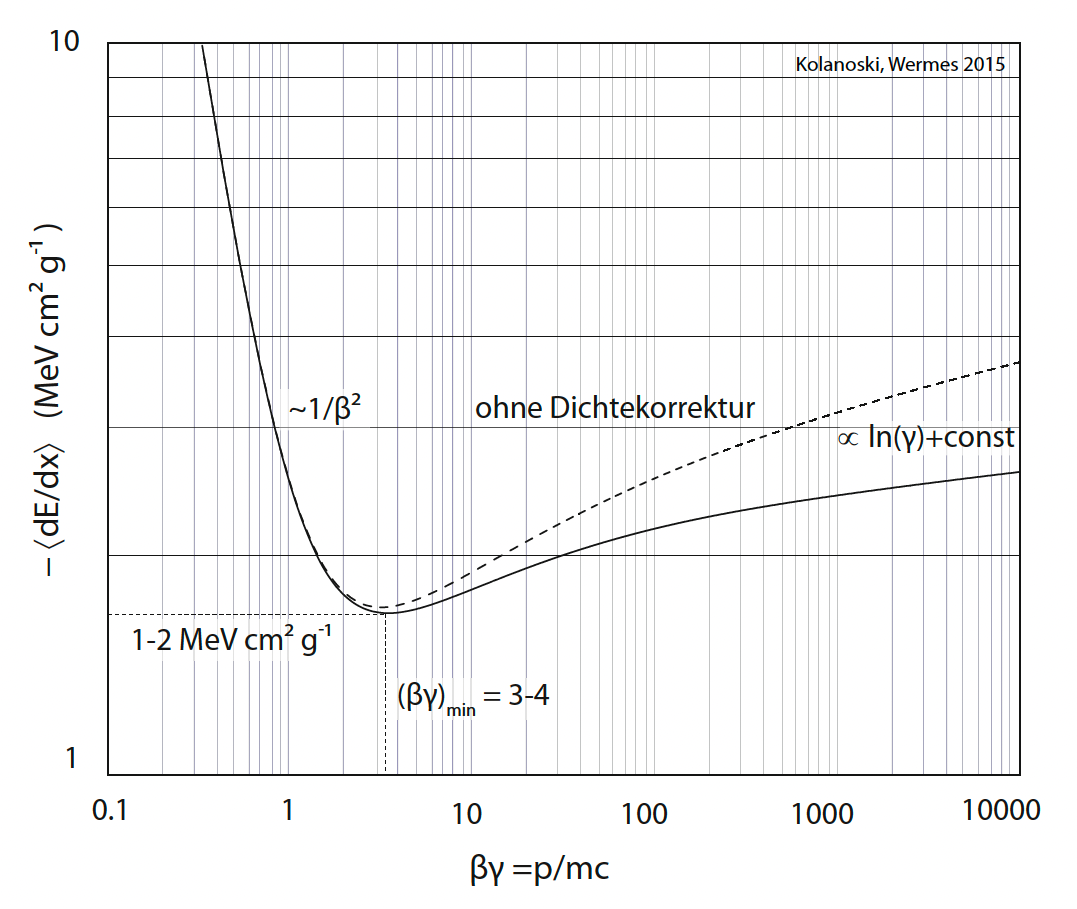
\includegraphics[width=0.7\linewidth]{img/bethe_curve.png}
	\caption{Verlauf des mittleren Energieverlusts von geladenen Teilchen in Materie als Funktion von $p/mc$. \cite{kolanoski} }
	\label{fig:bethecurve}
\end{figure}
%
%
\begin{figure}[h]
	\centering
	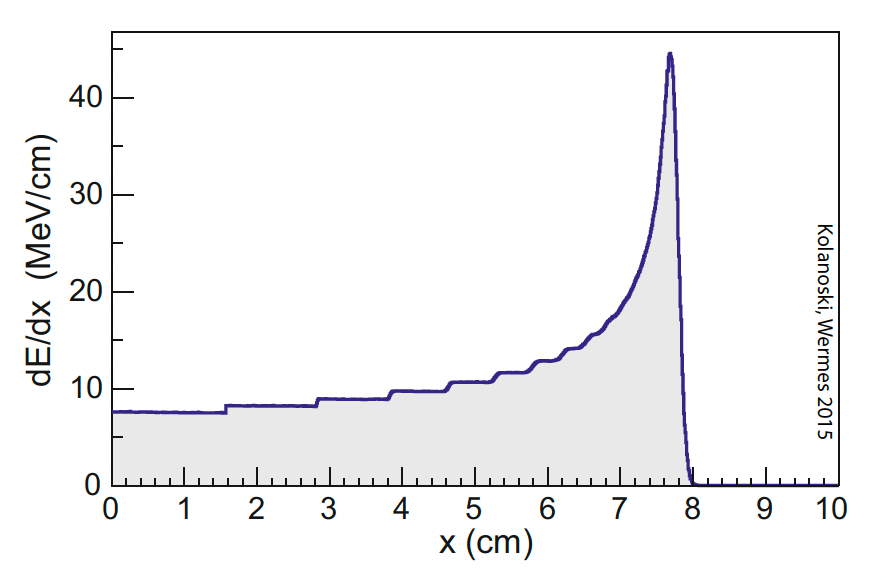
\includegraphics[width=0.7\linewidth]{img/bragg_peak.png}
	\caption{Bragg Peak. Energieverlust pro Wegstrecke als Funktion der bereits zurückgelegten Wegstrecke. Hier am Beispiel von Protonen in Wasser. \cite{kolanoski}}
	\label{fig:braggpeak}
\end{figure}
\FloatBarrier
%
\subsection{Halbleiterdetektoren}
Zum Nachweis von Alphastrahlung, beispielsweise zu Strahlenschutzzwecken, eignen sich im Prinzip alle Teilchendetektoren. Allerdings muss die Strahlung das Innere des Detektors, das empfindliche Volumen, erreichen können; ein Zählrohr muss dazu ein genügend dünnes Folienfenster haben. Für genaue Messungen, etwa zur Bestimmung des Energiespektrums der Strahlung, müssen sich Strahlenquelle und Detektor in einem gemeinsamen Vakuum befinden. Dabei wird meist ein Halbleiterdetektor verwendet. \cite{dewiki:240085809}

Im Grunde sind Silizium-Halbleiterdetektoren relativ große p-n-Halbleiterdioden mit einem sehr dünnen Eintrittsfenster für geladene Teilchen, das minimalem Energieverlust bietet. Sie werden in Sperrrichtung betrieben, sodass durch eine angelegte Spannung freie Ladungsträger aus dem sensitiven Volumen (Verarmungszone) der Diode gesaugt werden. Abbildung \ref{fig:surfacebarrier} zeigt den Aufbau des in diesem Experiment verwendeten Detektors. 

Wenn ein geladenes Teilchen, etwa ein Alpha-Teilchen, in den Detektor eindringt, verliert es einen geringen Teil seiner Energie am dünnen Eintrittsfenster. Der Großteil seiner Energie wird in der Verarmungszone durch Ionisation der Silizium-Atome deponiert. Die Anzahl der Elektron-Loch-Paare, welche durch diesen Prozess erzeugt werden, ist proportional zur Energie des einfallenden Teilchens. Die freie Ladung, erzeugt durch die Ionisation, wird von den Elektroden abgesaugt und mithilfe der Kondensatoren des über den Konnektor verbundenen Vorverstärkers aufgesammelt. Die gesammelte Ladung resultiert in einem Spannungspuls, welcher von der Kapazität des Vorverstärkers und der Ladungsmenge bestimmt ist und innerhalb von bis zu $100$~ns ansteigt. Die Amplitude des Spannungspulses ist proportional zur Energie des gemessenen Alpha-Teilchens und kann mithilfe eines Vielkanal-Impulshöhen-Analysators (MCA) zur Auswertung weiterverarbeitet werden.

\begin{figure}[h]
	\centering
	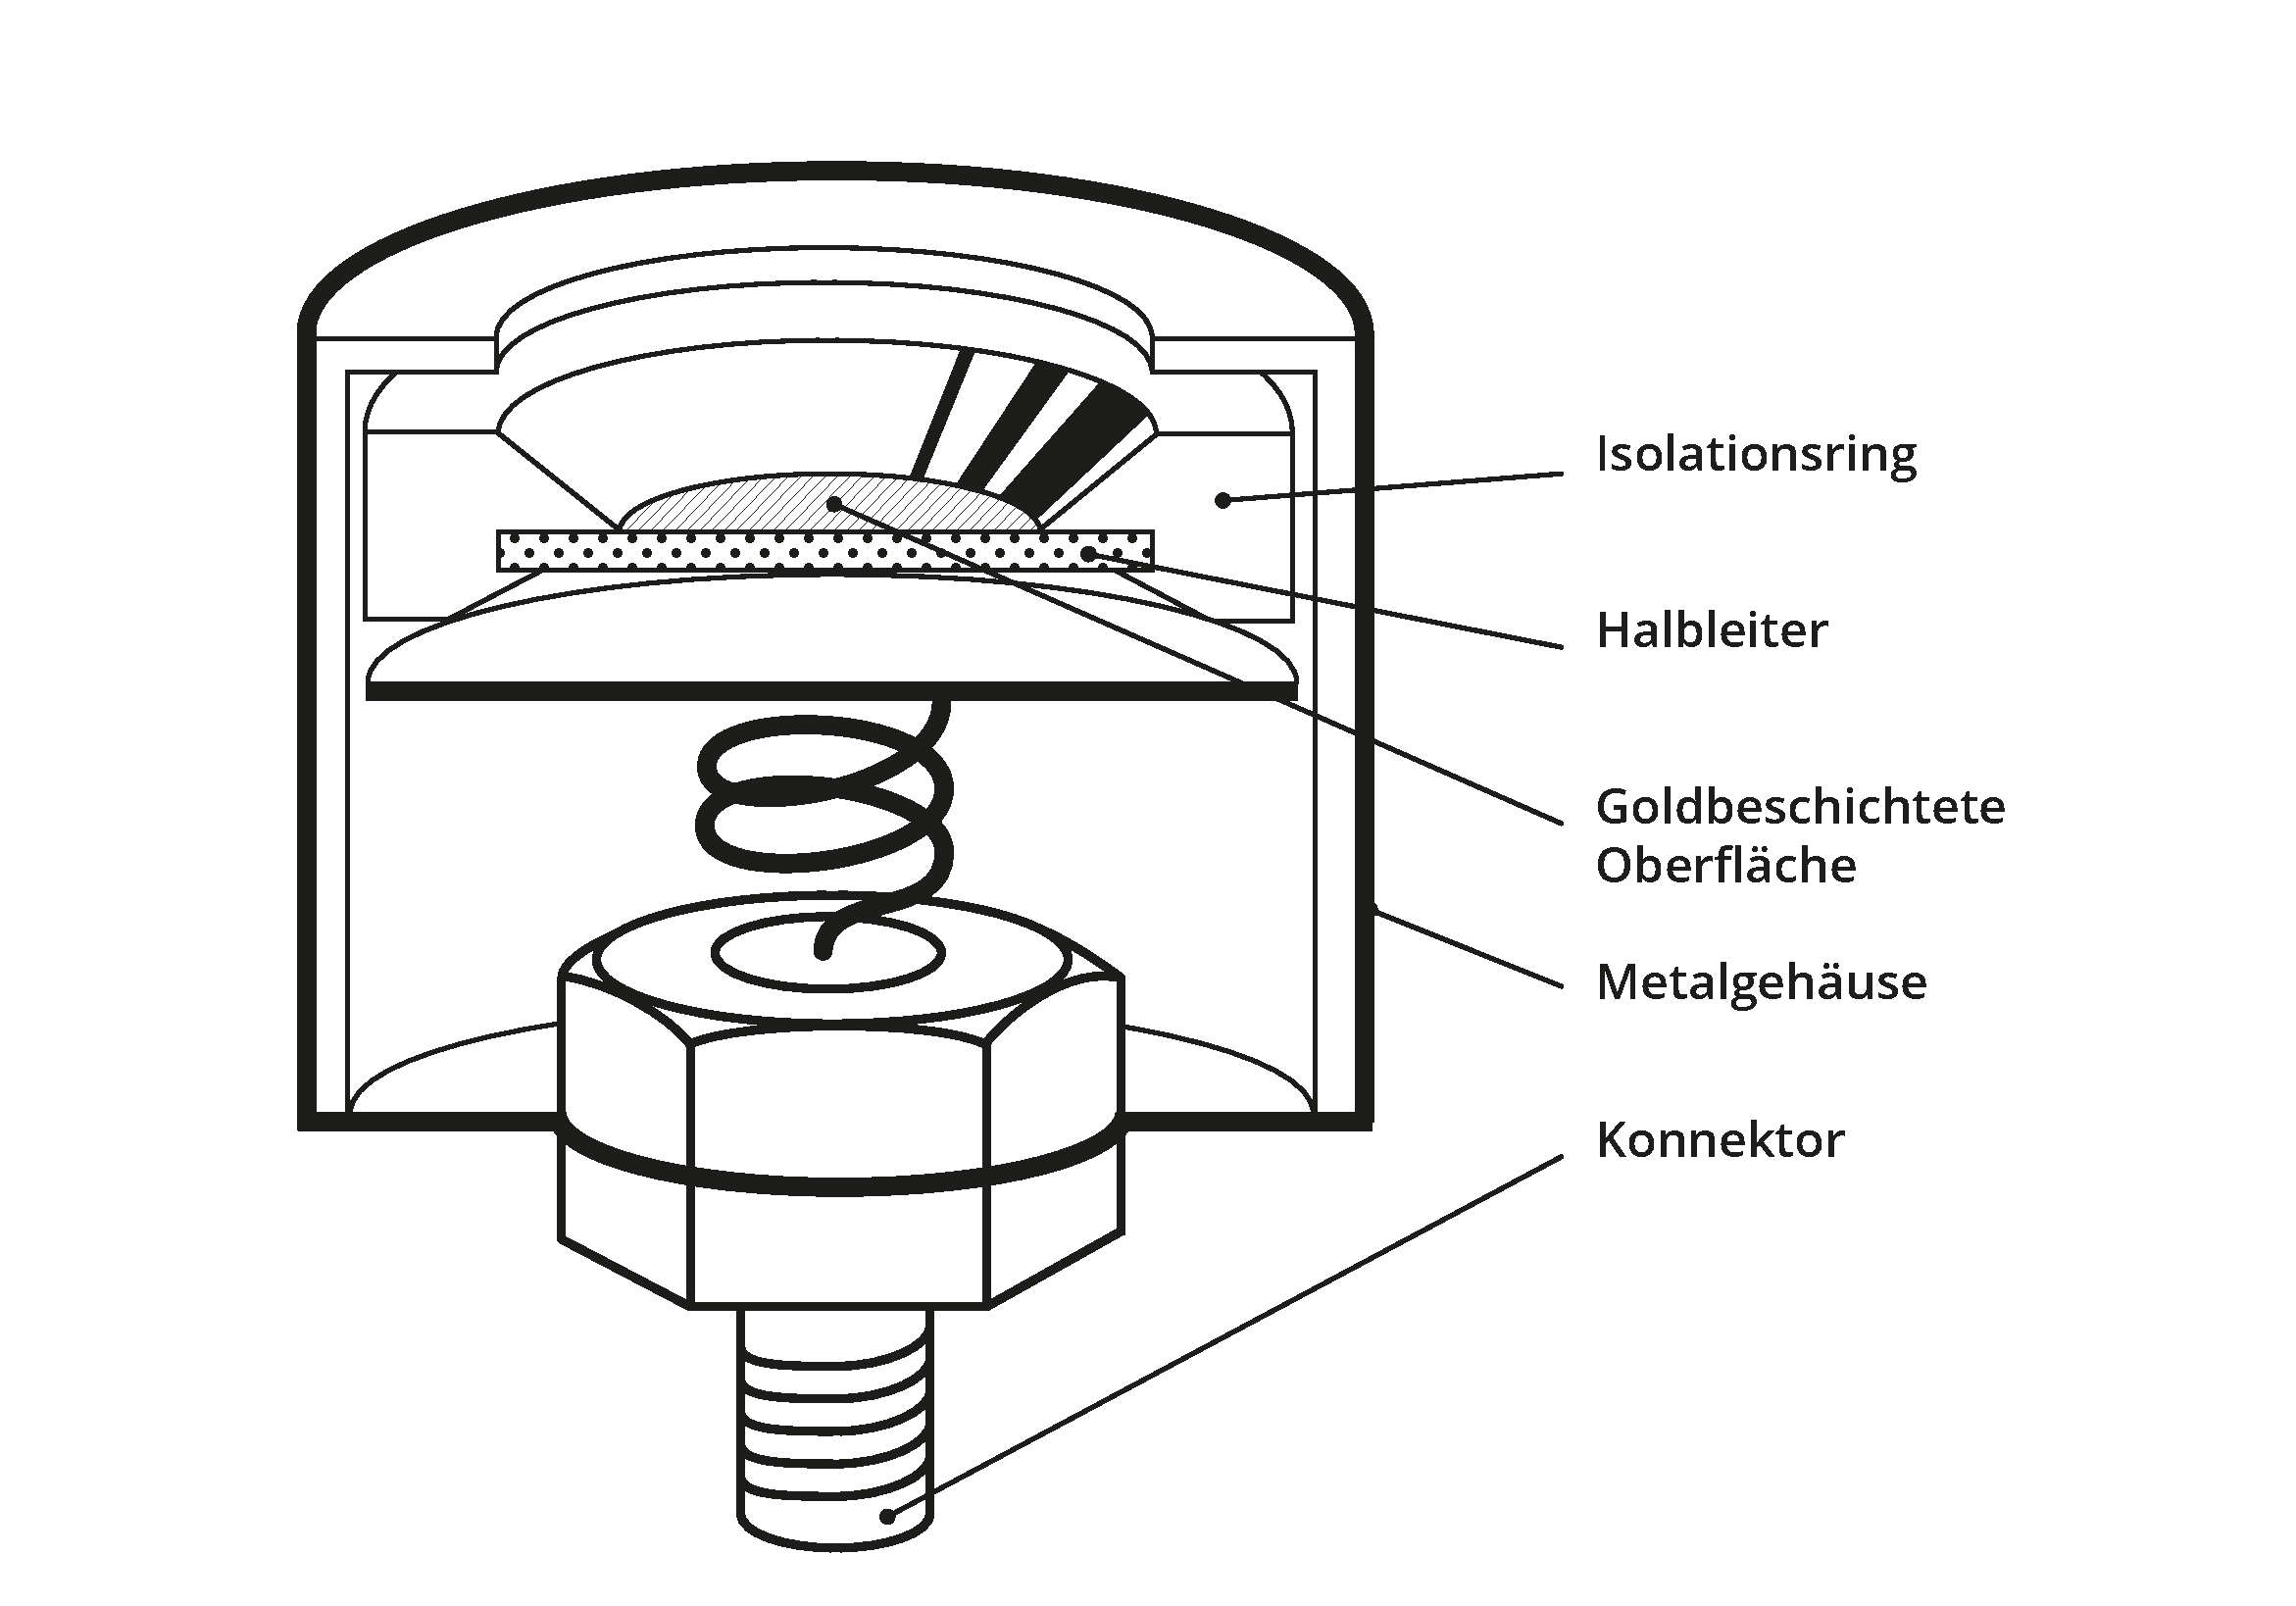
\includegraphics[width=0.7\linewidth]{img/surface_barrier}
	\caption{Aufbau des Oberflächensperrschichtzählers \cite{leo}.}
	\label{fig:surfacebarrier}
\end{figure}

Halbleiterdetektoren können in einem großflächigen Energiebereich für Elektronen mit etwa 20~keV bis zu schweren Ionen mit 200~MeV eingesetzt werden. Die Effizienz von Halbleiterdetektoren im aktiven Volumen beträgt annähernd 100\%, während die Proportionalität von der Energie geladener Teilchen zur Pulshöhe über einen weiten Bereich konstant ist. Durch den weitverbreiteten Einsatz von Siliziumtransistoren sind die verwendeten Halbleiterdetektoren zudem noch sehr kostengünstig.

\paragraph{Themen zur Vorbereitung}
\begin{itemize}
	\item Halbleiter, Dotierung, Diode, p-n-Übergang, Diffusionsspannung.
	\item Energiedeposition, Bildung und Rekombination von Ladungsträgern.
	\item Energieauflösung des Halbleiterdetektors.
	\item Thermisches Rauschen, Energie pro Elektron-Loch-Paar.
	\item Poisson Statistik, Fano-Faktor (siehe \cite[Kap. 17.10.2]{kolanoski})
\end{itemize}

%\begin{figure}
%	\begin{center}
%		\includegraphics[0.95\textwidth]{figs/signal_chain.pdf}
%		\caption{Verkabelung} \label{fig:verkabelung}
%	\end{center}
%\end{figure}

%\subsection{Signalverarbeitung}
% details Signalverarbeitung :
% was macht der Vorverstaerker
% was macht der Hauptverstaerker
% was macht der ADC
% was ist ein Vielkanalanalysator, was ist ein Kanal

% Bildliche Darstellungen
\clearpage
\section{Versuchsaufbau}
Der Versuchsaufbau besteht aus folgenden Komponenten:
\begin{itemize}
	\item Strahlungsquelle
	\item Halbleiterdetektor
	\item Vakuumgefäß mit Manometer, Ein- und Auslassventil
	\item Vakuumpumpe
	\item Vorverstärker und Hauptverstärker für die Detektorsignale
	\item Spannungsversorgungsgerät mit externem Spannungsmessgerät
	\item Vielkanalpulshöhenanalysator (Multi Channel Analysator -- MCA)\\im PC
	\item PC mit MCA-Software
\end{itemize}

Abbildung \ref{fig:aufbauhalbleiter} zeigt den Versuchsaufbau schematisch, Fotos sind in Abbildung \ref{fig:setup_} zu sehen. Der Oberflächensperrschichtzähler und die Alphastrahlungsquelle befinden sich in einem luftdichten Metallzylinder. Die Quelle lässt sich im Zylinder entlang einer Raumachse verschieben, um den Abstand zwischen Quelle und Detektor verändern zu können. Bei minimalem einstellbaren Abstand berühren sich Quelle und Detektor nicht, die Bestimmung dieses Nullabstandes ist Teil des Versuchs.
\begin{figure}[h]
	\centering
	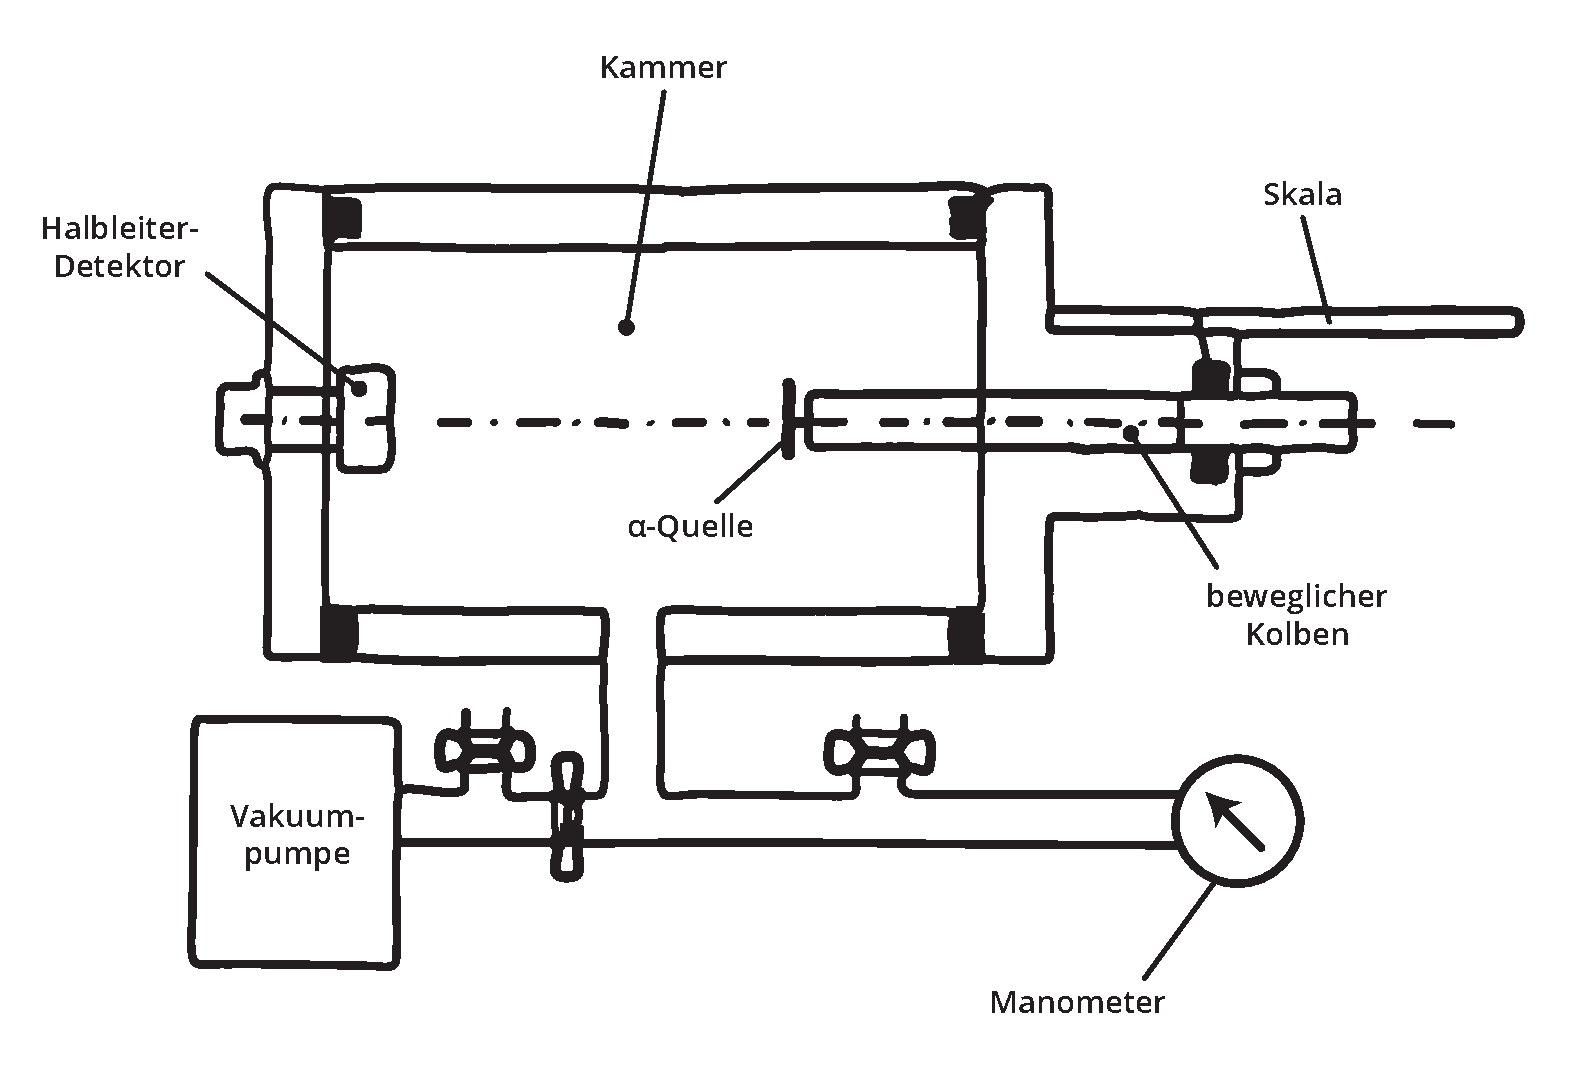
\includegraphics[width=0.7\linewidth]{img/aufbau_halbleiter}
	\caption{Versuchsaufbau}
	\label{fig:aufbauhalbleiter}
\end{figure}

Die Mischquelle hat einen aktiven Bereich mit einem Durchmesser von circa 7~mm und ist durch eine etwa 2~\textmu m dicke Goldschicht abgedeckt (siehe Abb. \ref{fig:quellefoto}). Die Abdeckung des radioaktiven Materials bietet bei Kontakt keinen Schutz vor Kontamination, deshalb muss die Quelle als offen angesehen werden. Für den Umgang mit offenen Quellen sind besondere Genehmigungsauflagen und Vorsichtsmaßnahmen zu beachten (siehe Abschnitt \ref{sec:warnhinweise}).

An den Halbleiterdetektor ist direkt außerhalb des Vakuumkolbens der Vorverstärker angebracht. Das Eintrittsfenster des Detektors ist in Abbildung \ref{fig:detektorfoto} zu sehen. Der Vorverstärker besitzt mehrere Anschlüsse: 
\begin{itemize}[itemsep=0pt]
	\item Versorgung Betriebsspannung, angeschlossen an der Rückseite des Hauptverstärkers. 
	\item Signalausgang, verbunden mit Signaleingang des Hauptverstärkers.
	\item Eingang externe Spannung, verbunden mit Spannungsversorgungsgerät.
	\item Anschlussmöglichkeit für einen Pulser. Nicht verbunden.
\end{itemize}
Die Verkabelung des Versuches ist in Abbildung \ref{fig:verkabelung} dargestellt und Abbildung \ref{fig:setup3} zeigt ein Foto des Hauptverstärkers sowie des Spannungsversorgungsgerätes.
%
\begin{figure}[h]
	\centering
	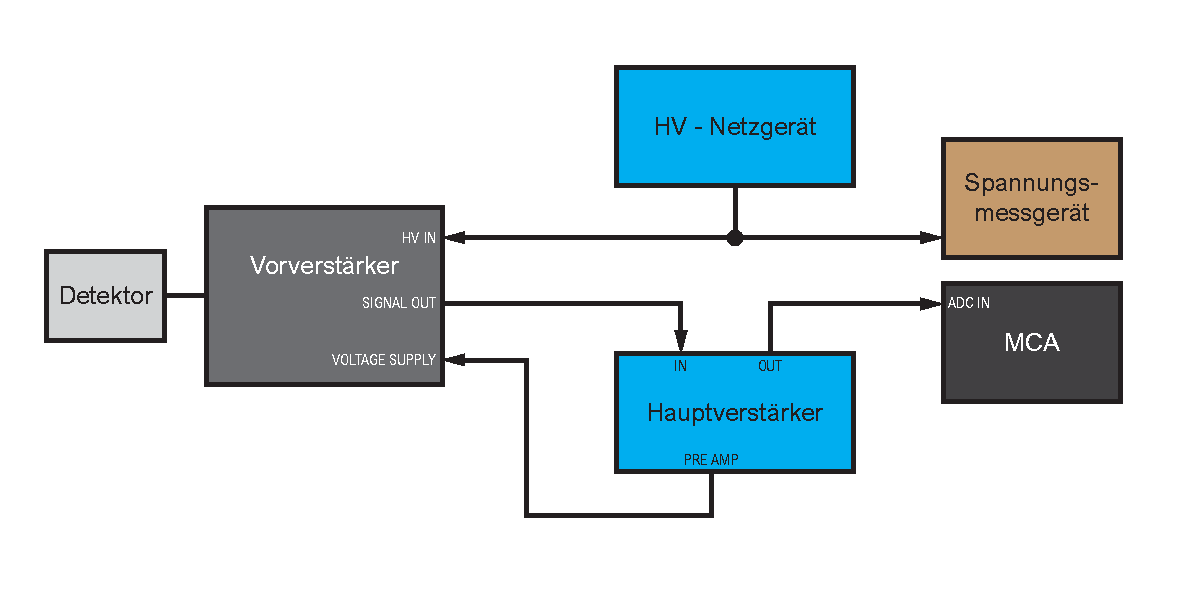
\includegraphics[width=\linewidth]{img/verkabelung}
	\caption{Schematische Darstellung der Verkabelung}
	\label{fig:verkabelung}
\end{figure}

\begin{figure}
	\centering
	\subcaptionbox{Ansicht von links. \label{fig:setup1}}[.49\linewidth]{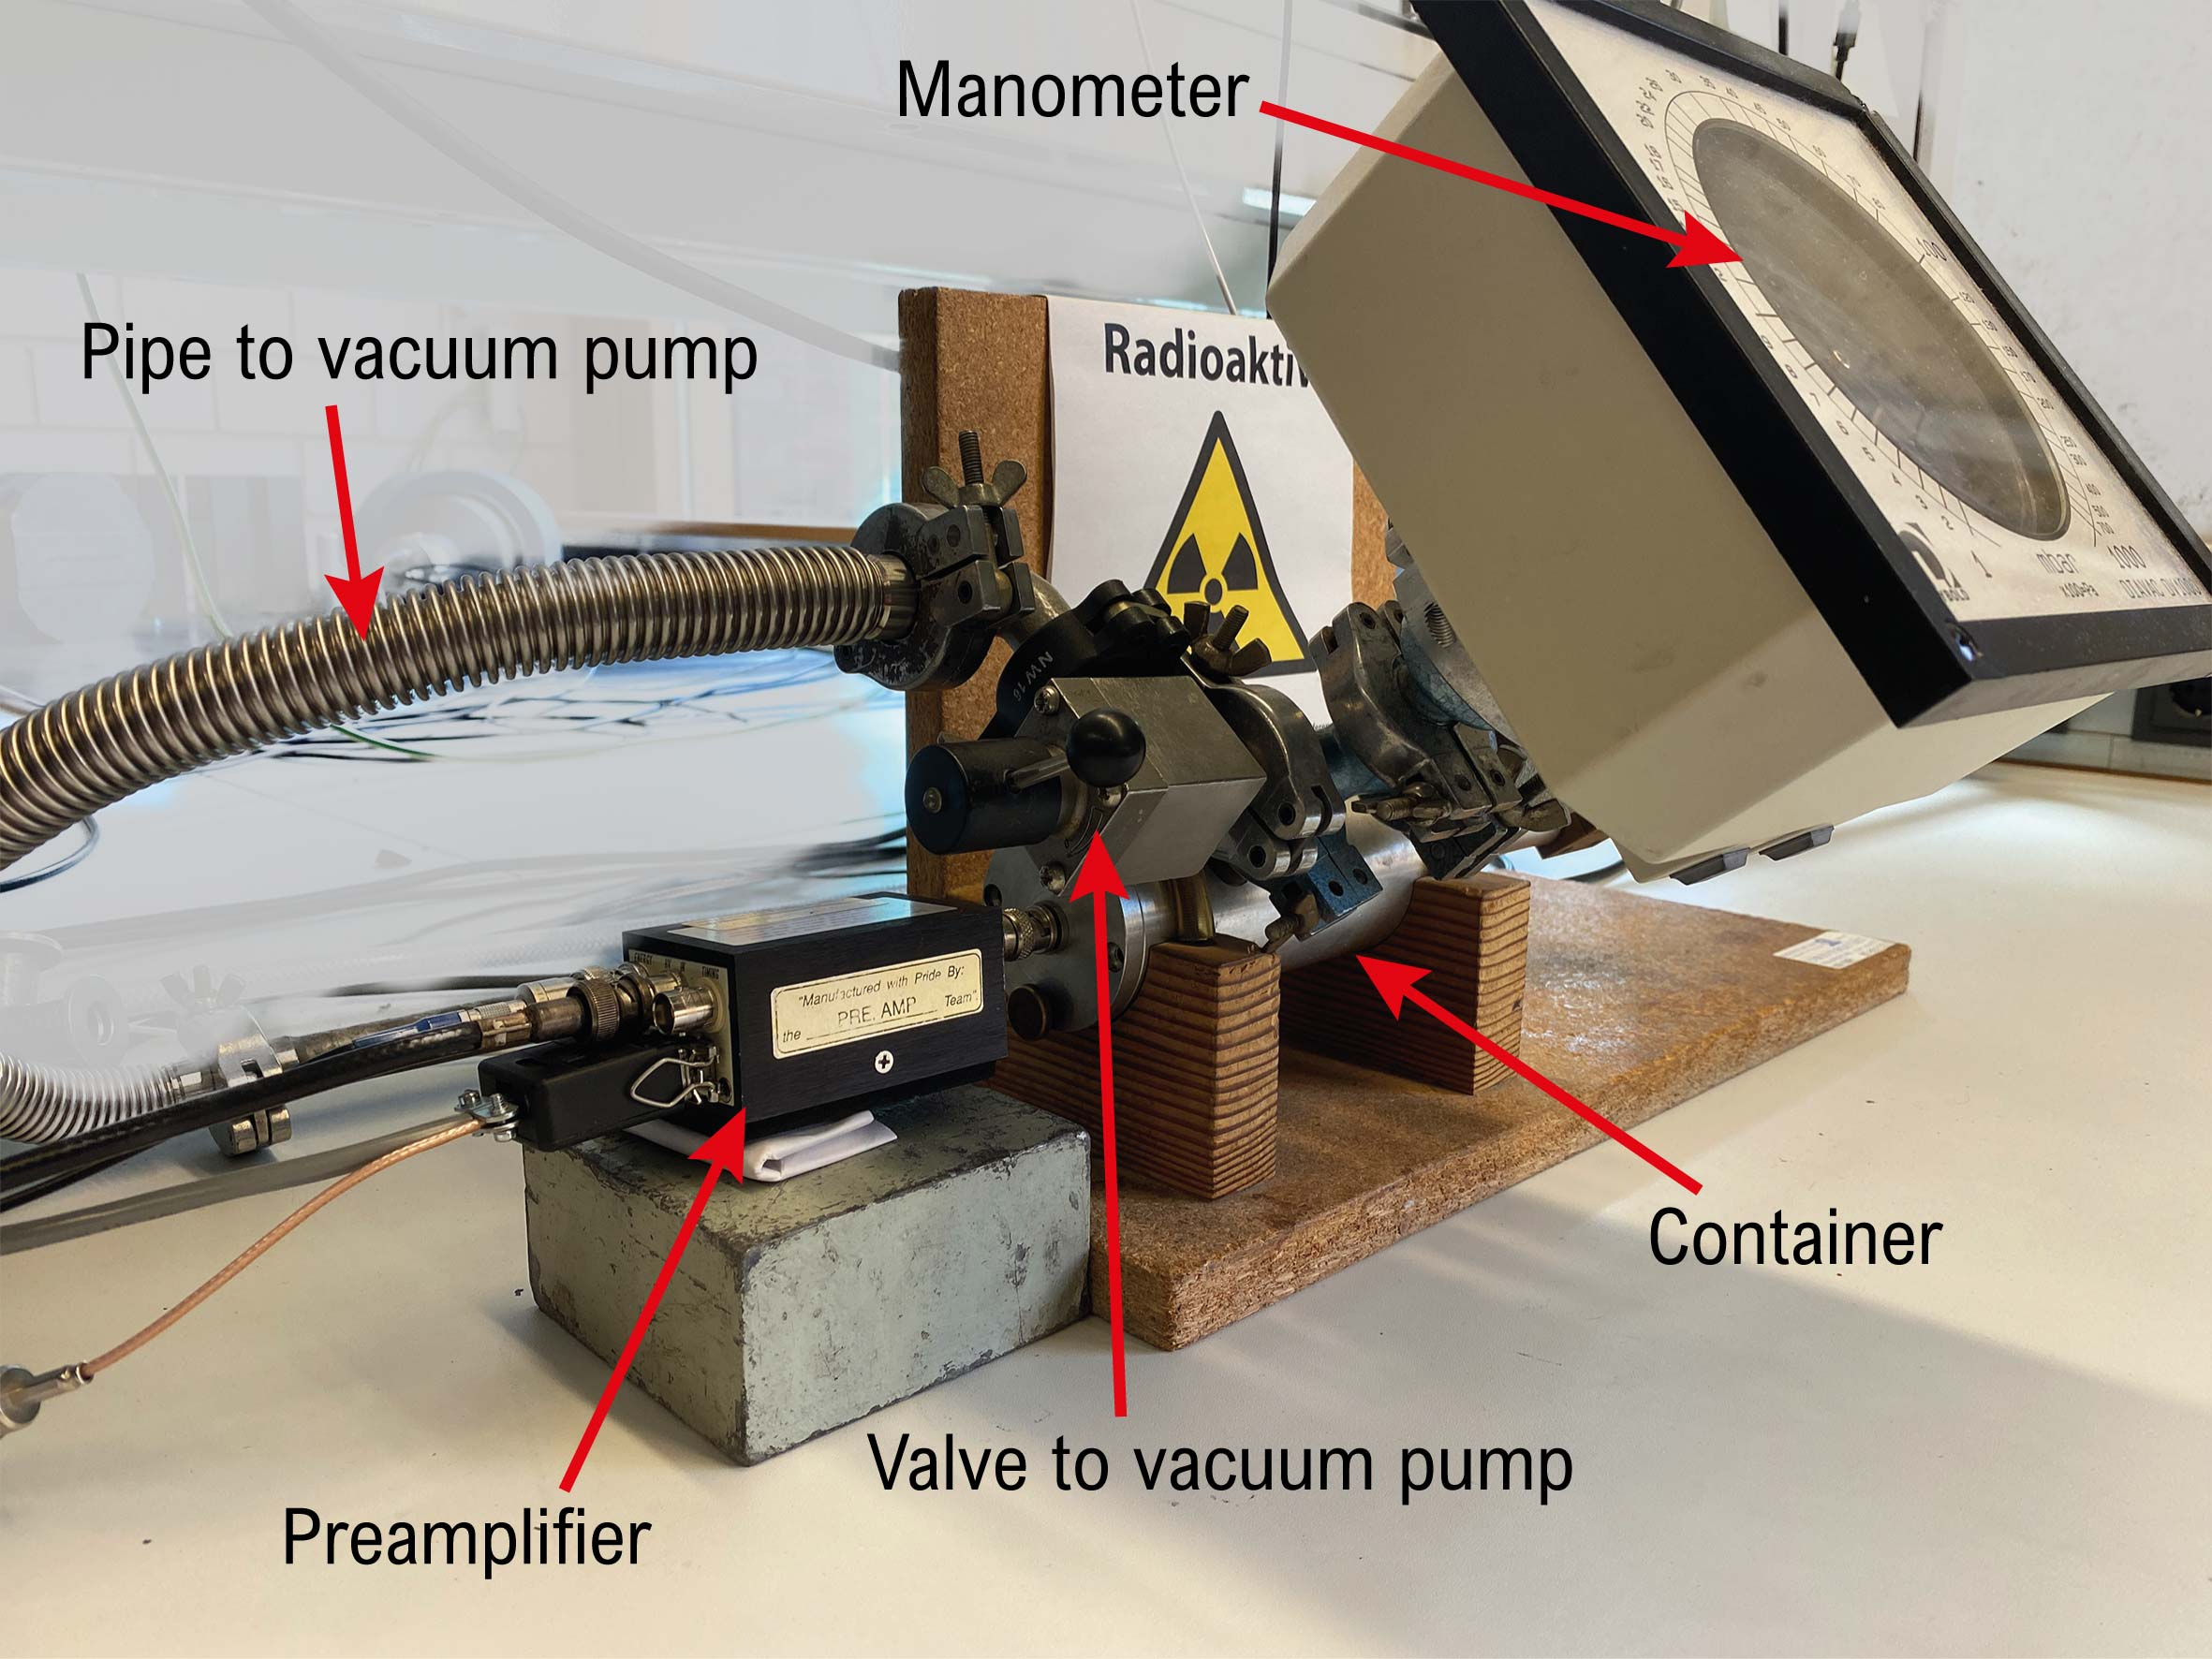
\includegraphics[width=\linewidth]{img/setup_1.jpg}}
	\subcaptionbox{Ansicht von rechts. \label{fig:setup2}}[.49\linewidth]{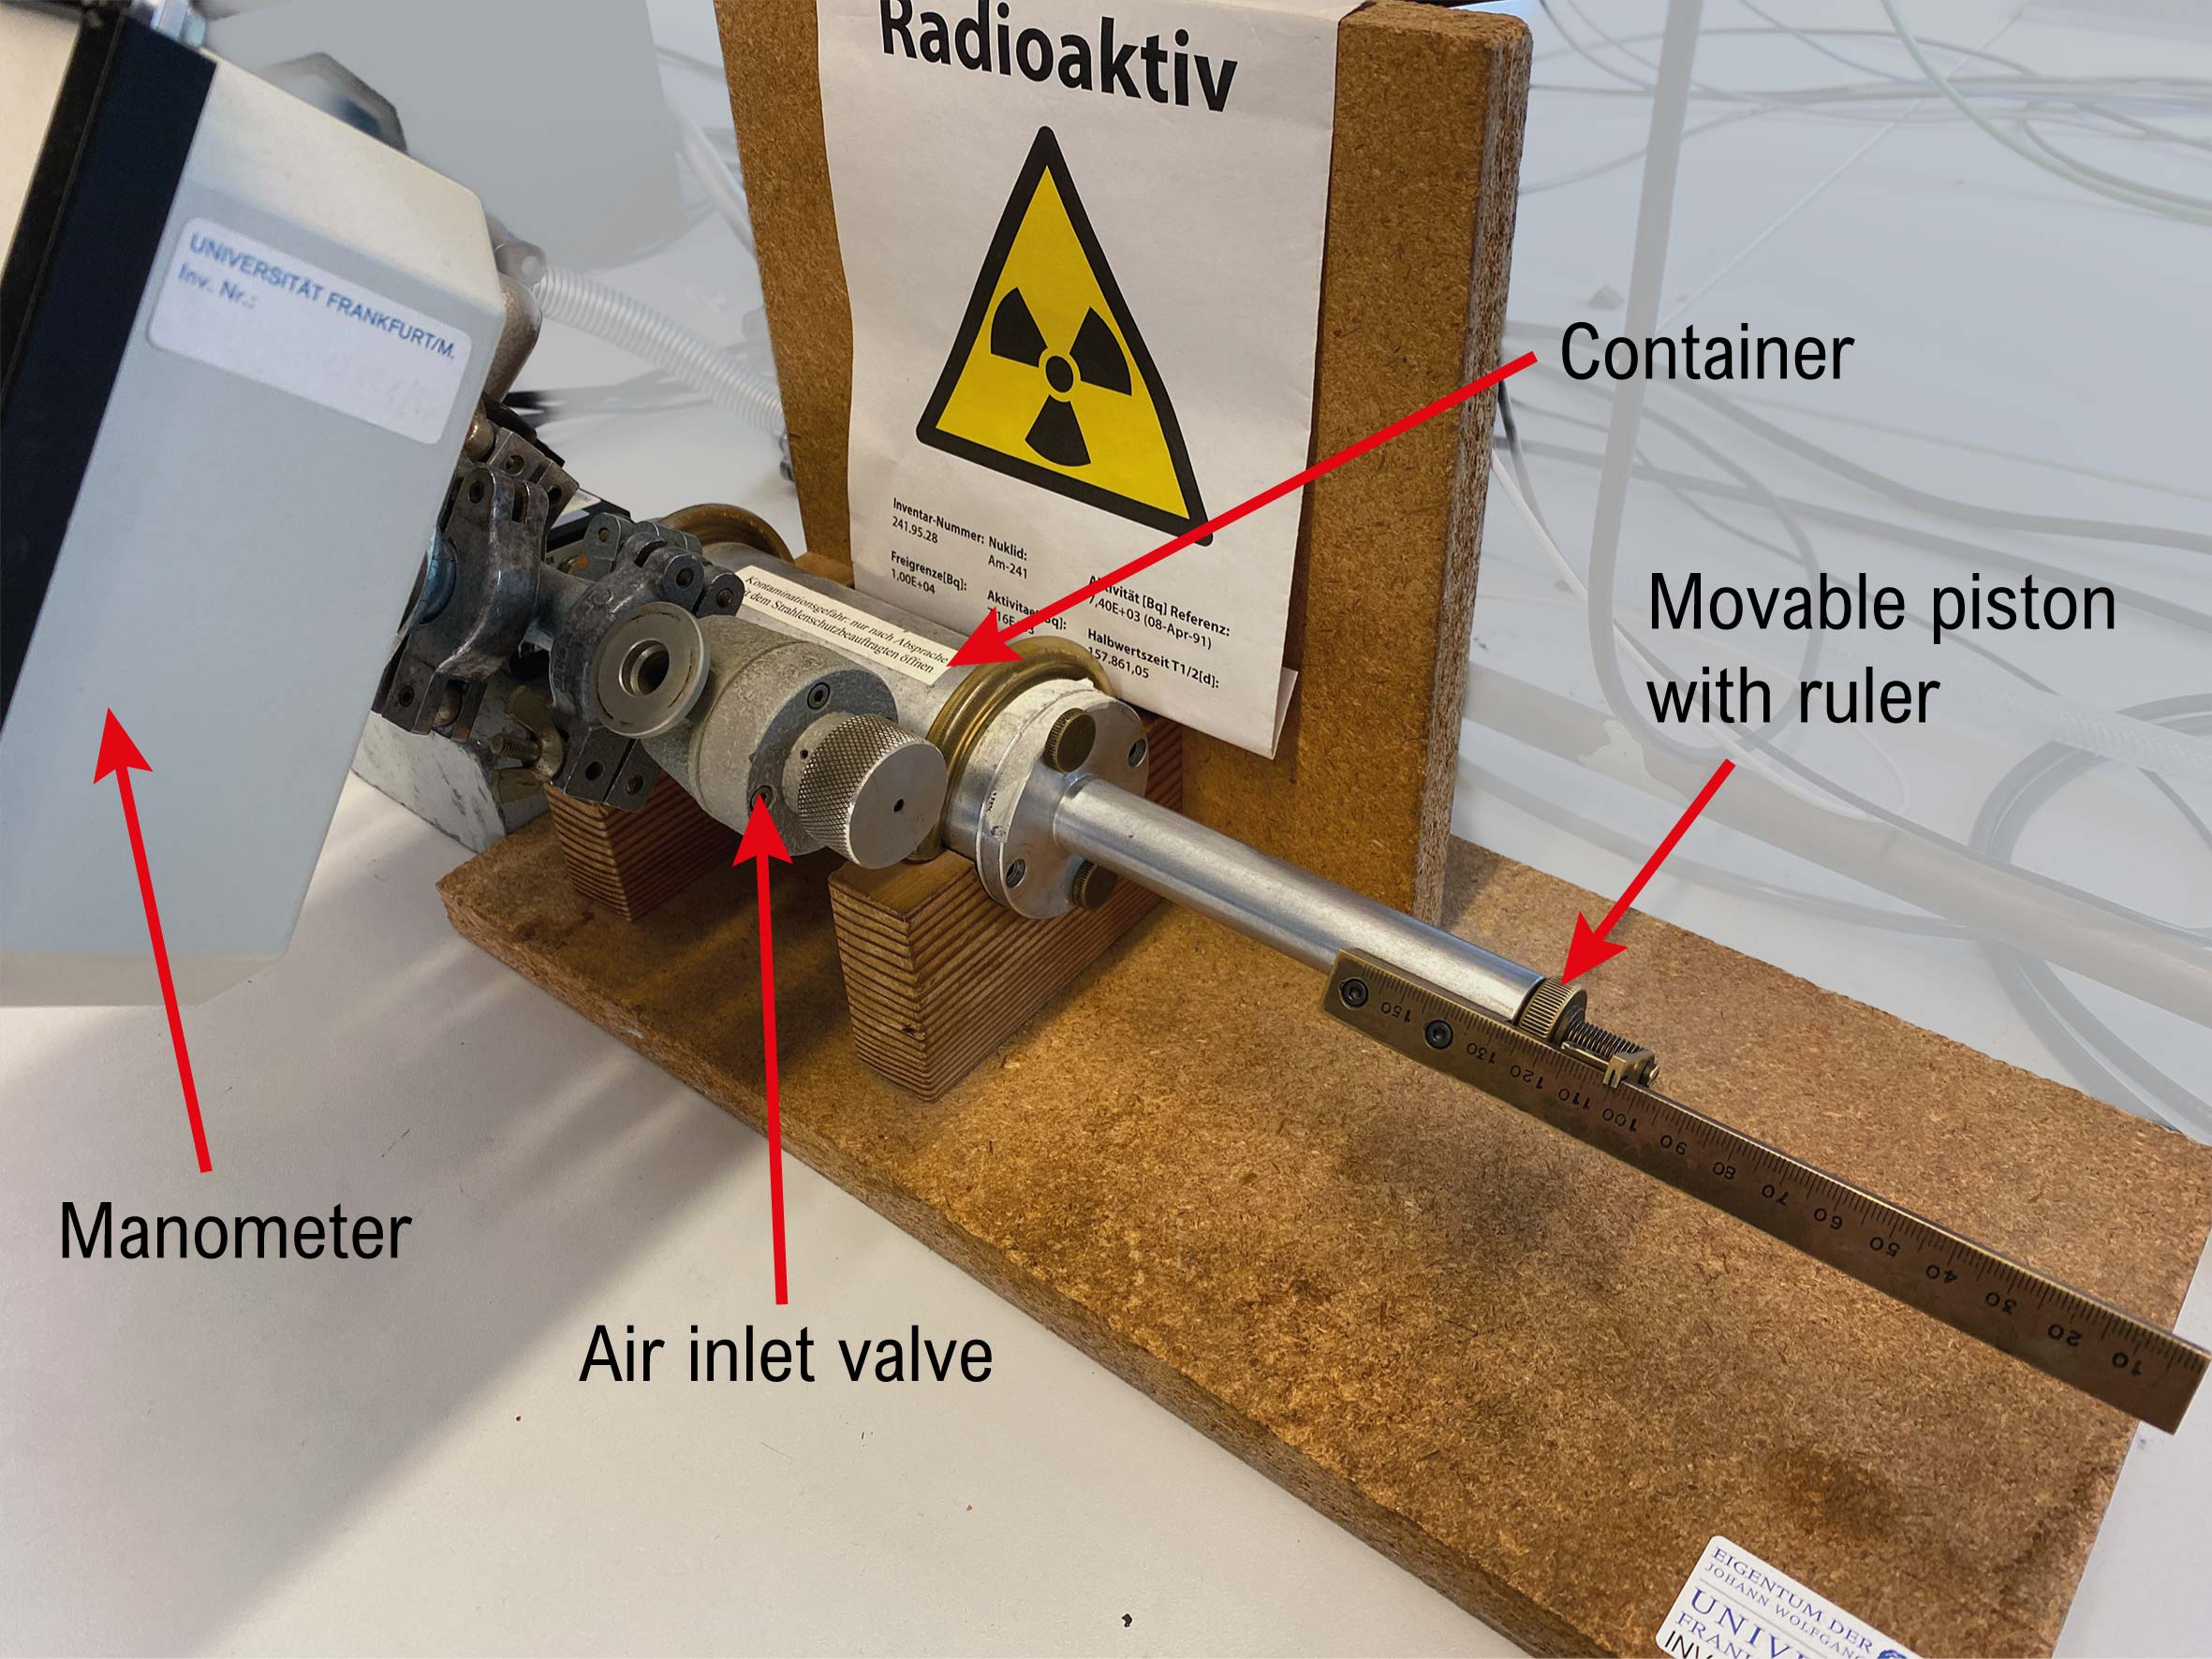
\includegraphics[width=\linewidth]{img/setup_2.jpg}}
	\caption{Der Versuchsaufbau}
	\label{fig:setup_}
\end{figure}
\begin{figure}
	\centering
	\subcaptionbox{Der Halbleiterdetektor. \label{fig:detektorfoto}}[.49\linewidth]
	{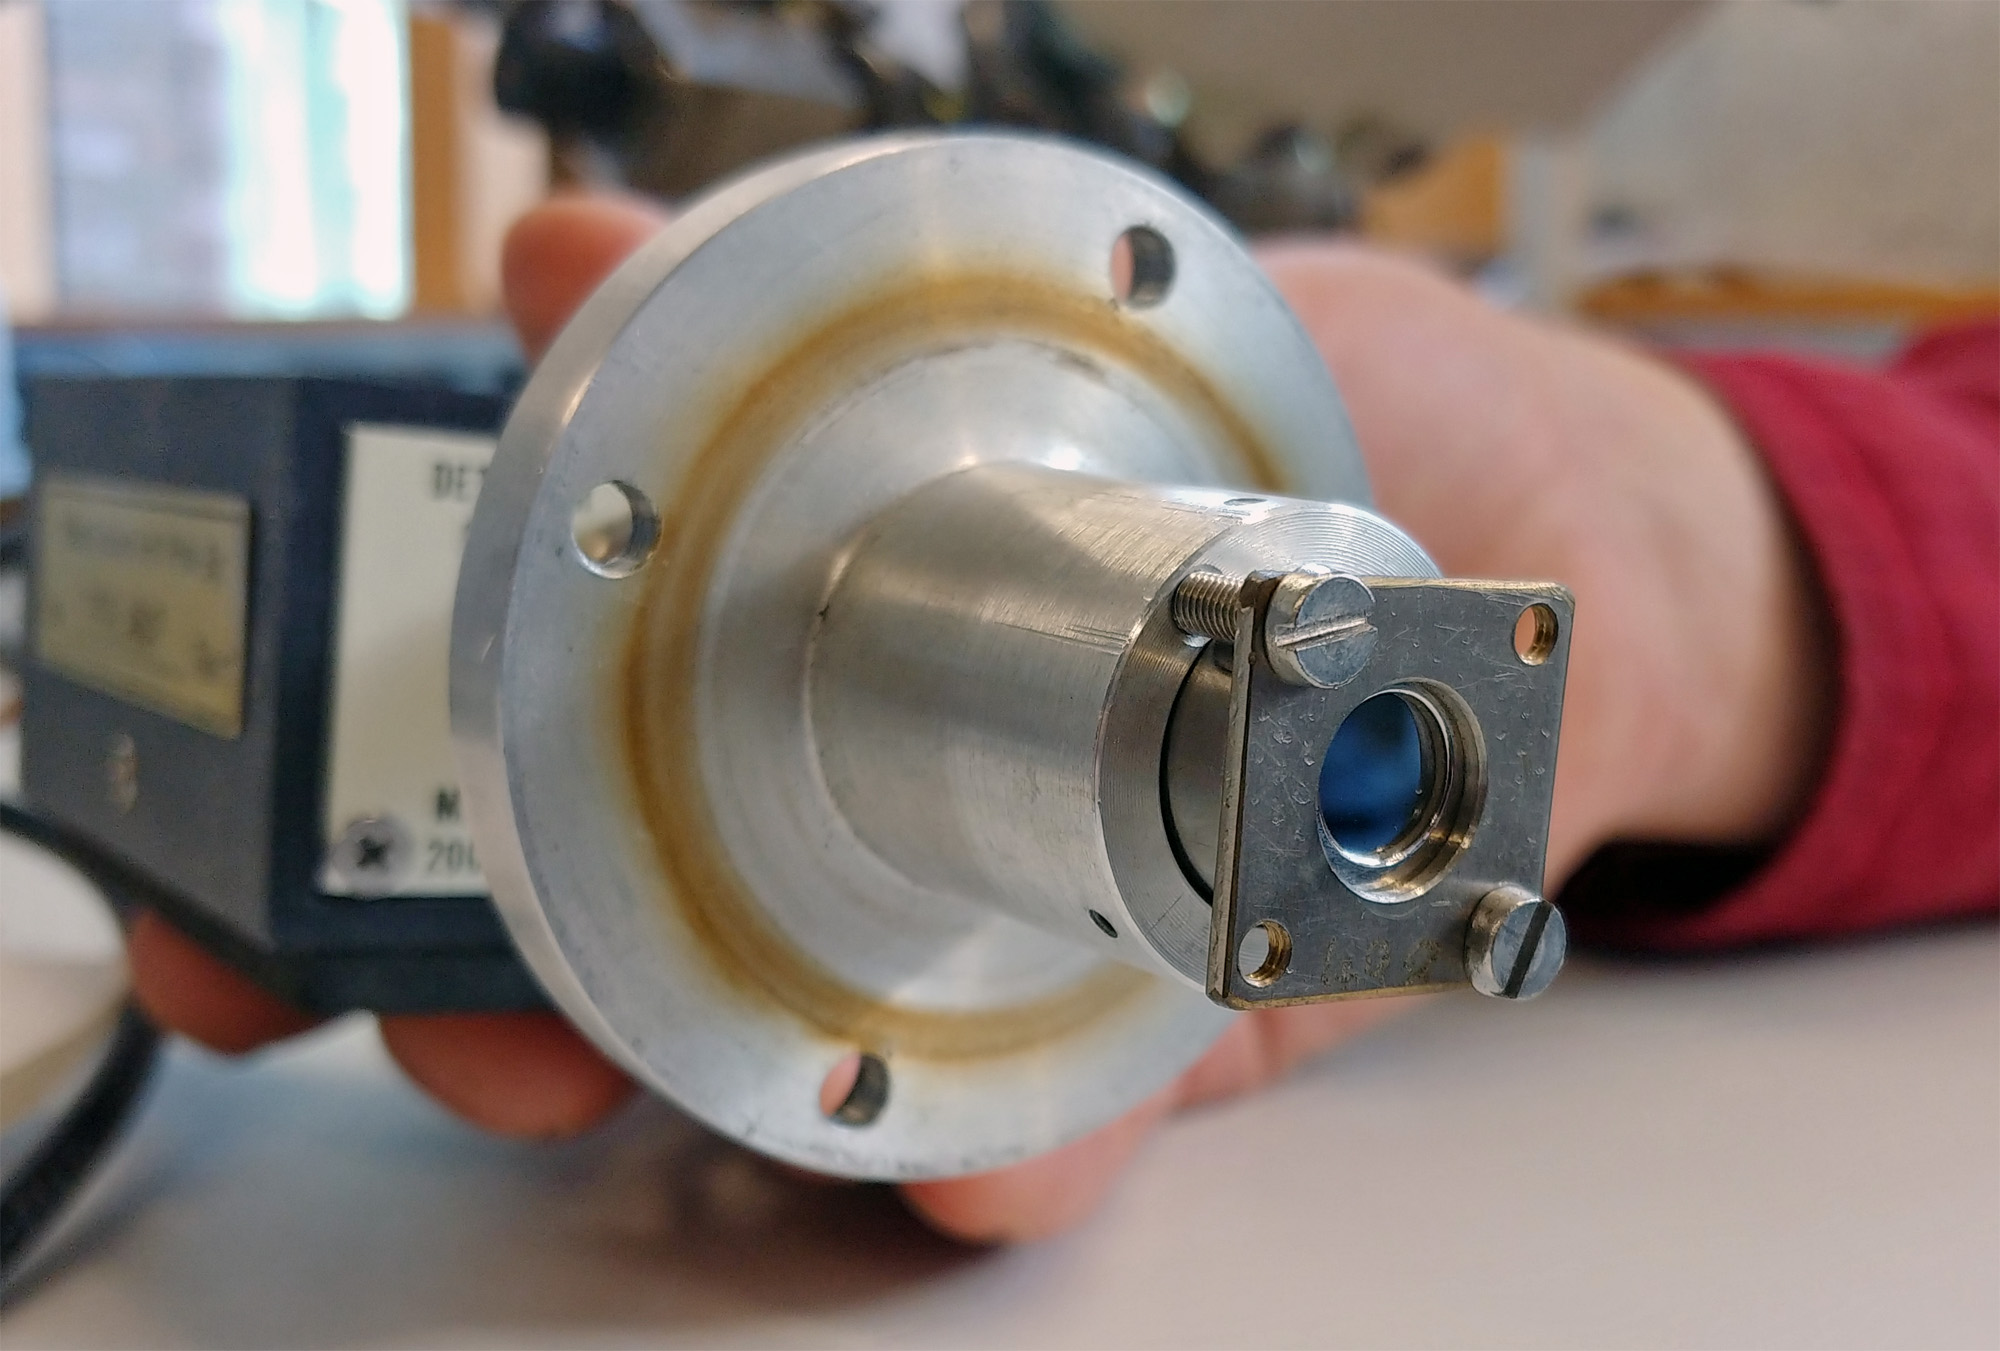
\includegraphics[width=\linewidth]{img/detektor_foto}}
	\subcaptionbox{Die Mischquelle mit goldener Oberfläche. \label{fig:quellefoto}}[.49\linewidth]
	{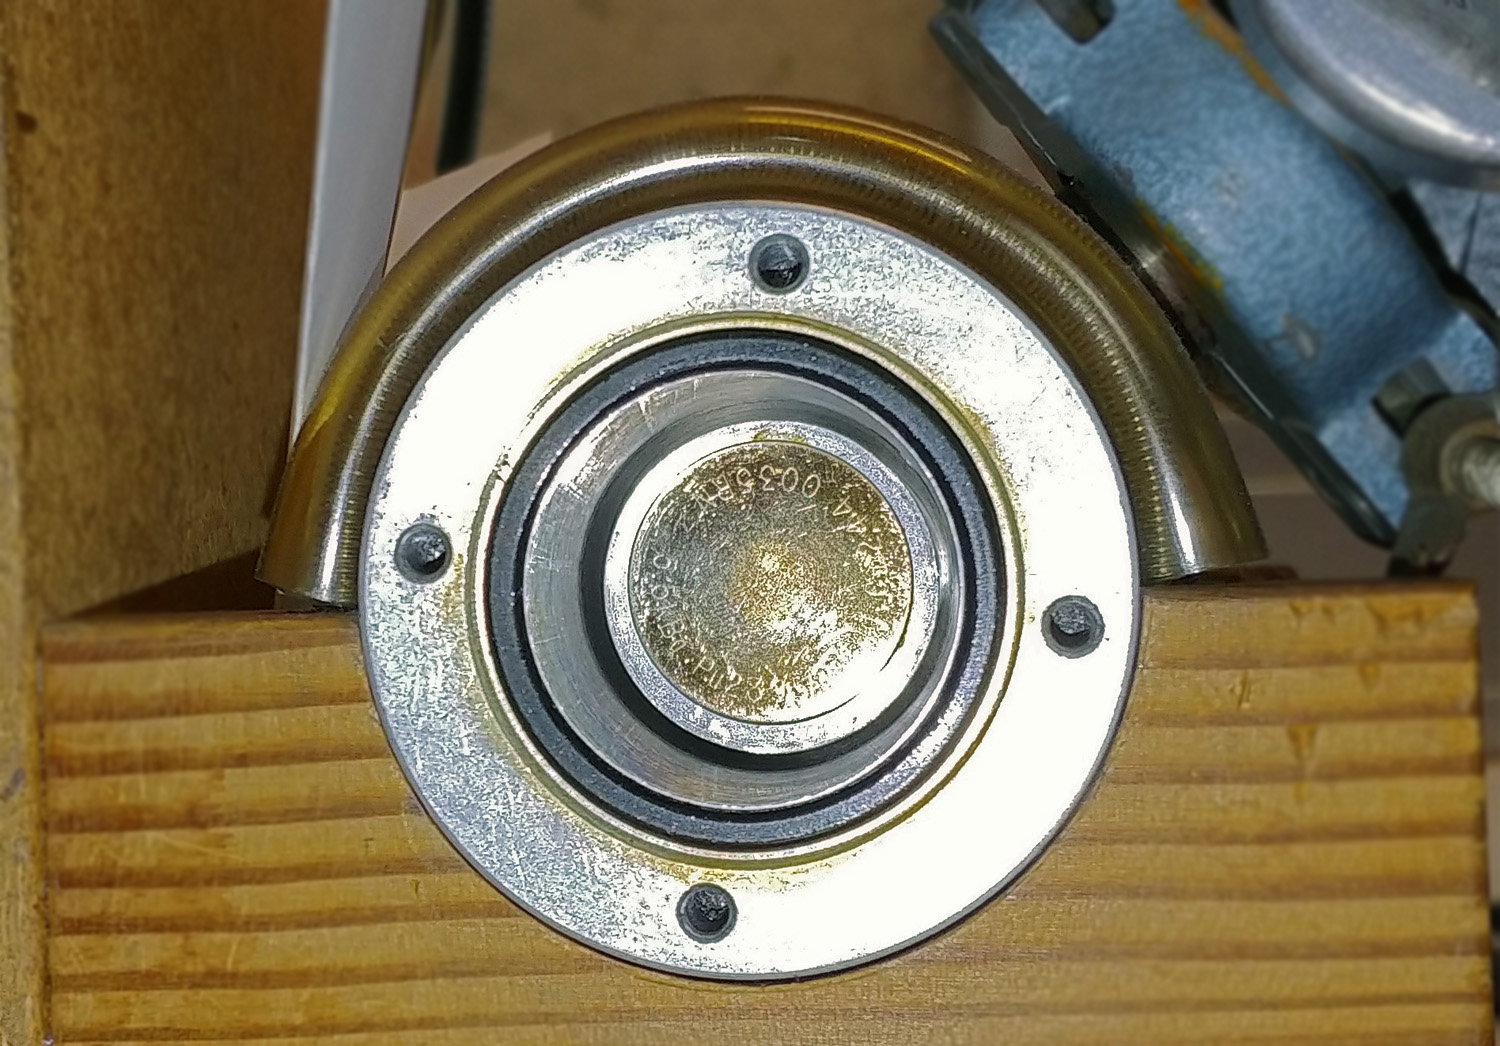
\includegraphics[width=\linewidth]{img/quelle_foto}}
	\caption{Innenansichten des Vakuumgefäßes (Container).}
\end{figure}
\begin{figure}
	\centering
	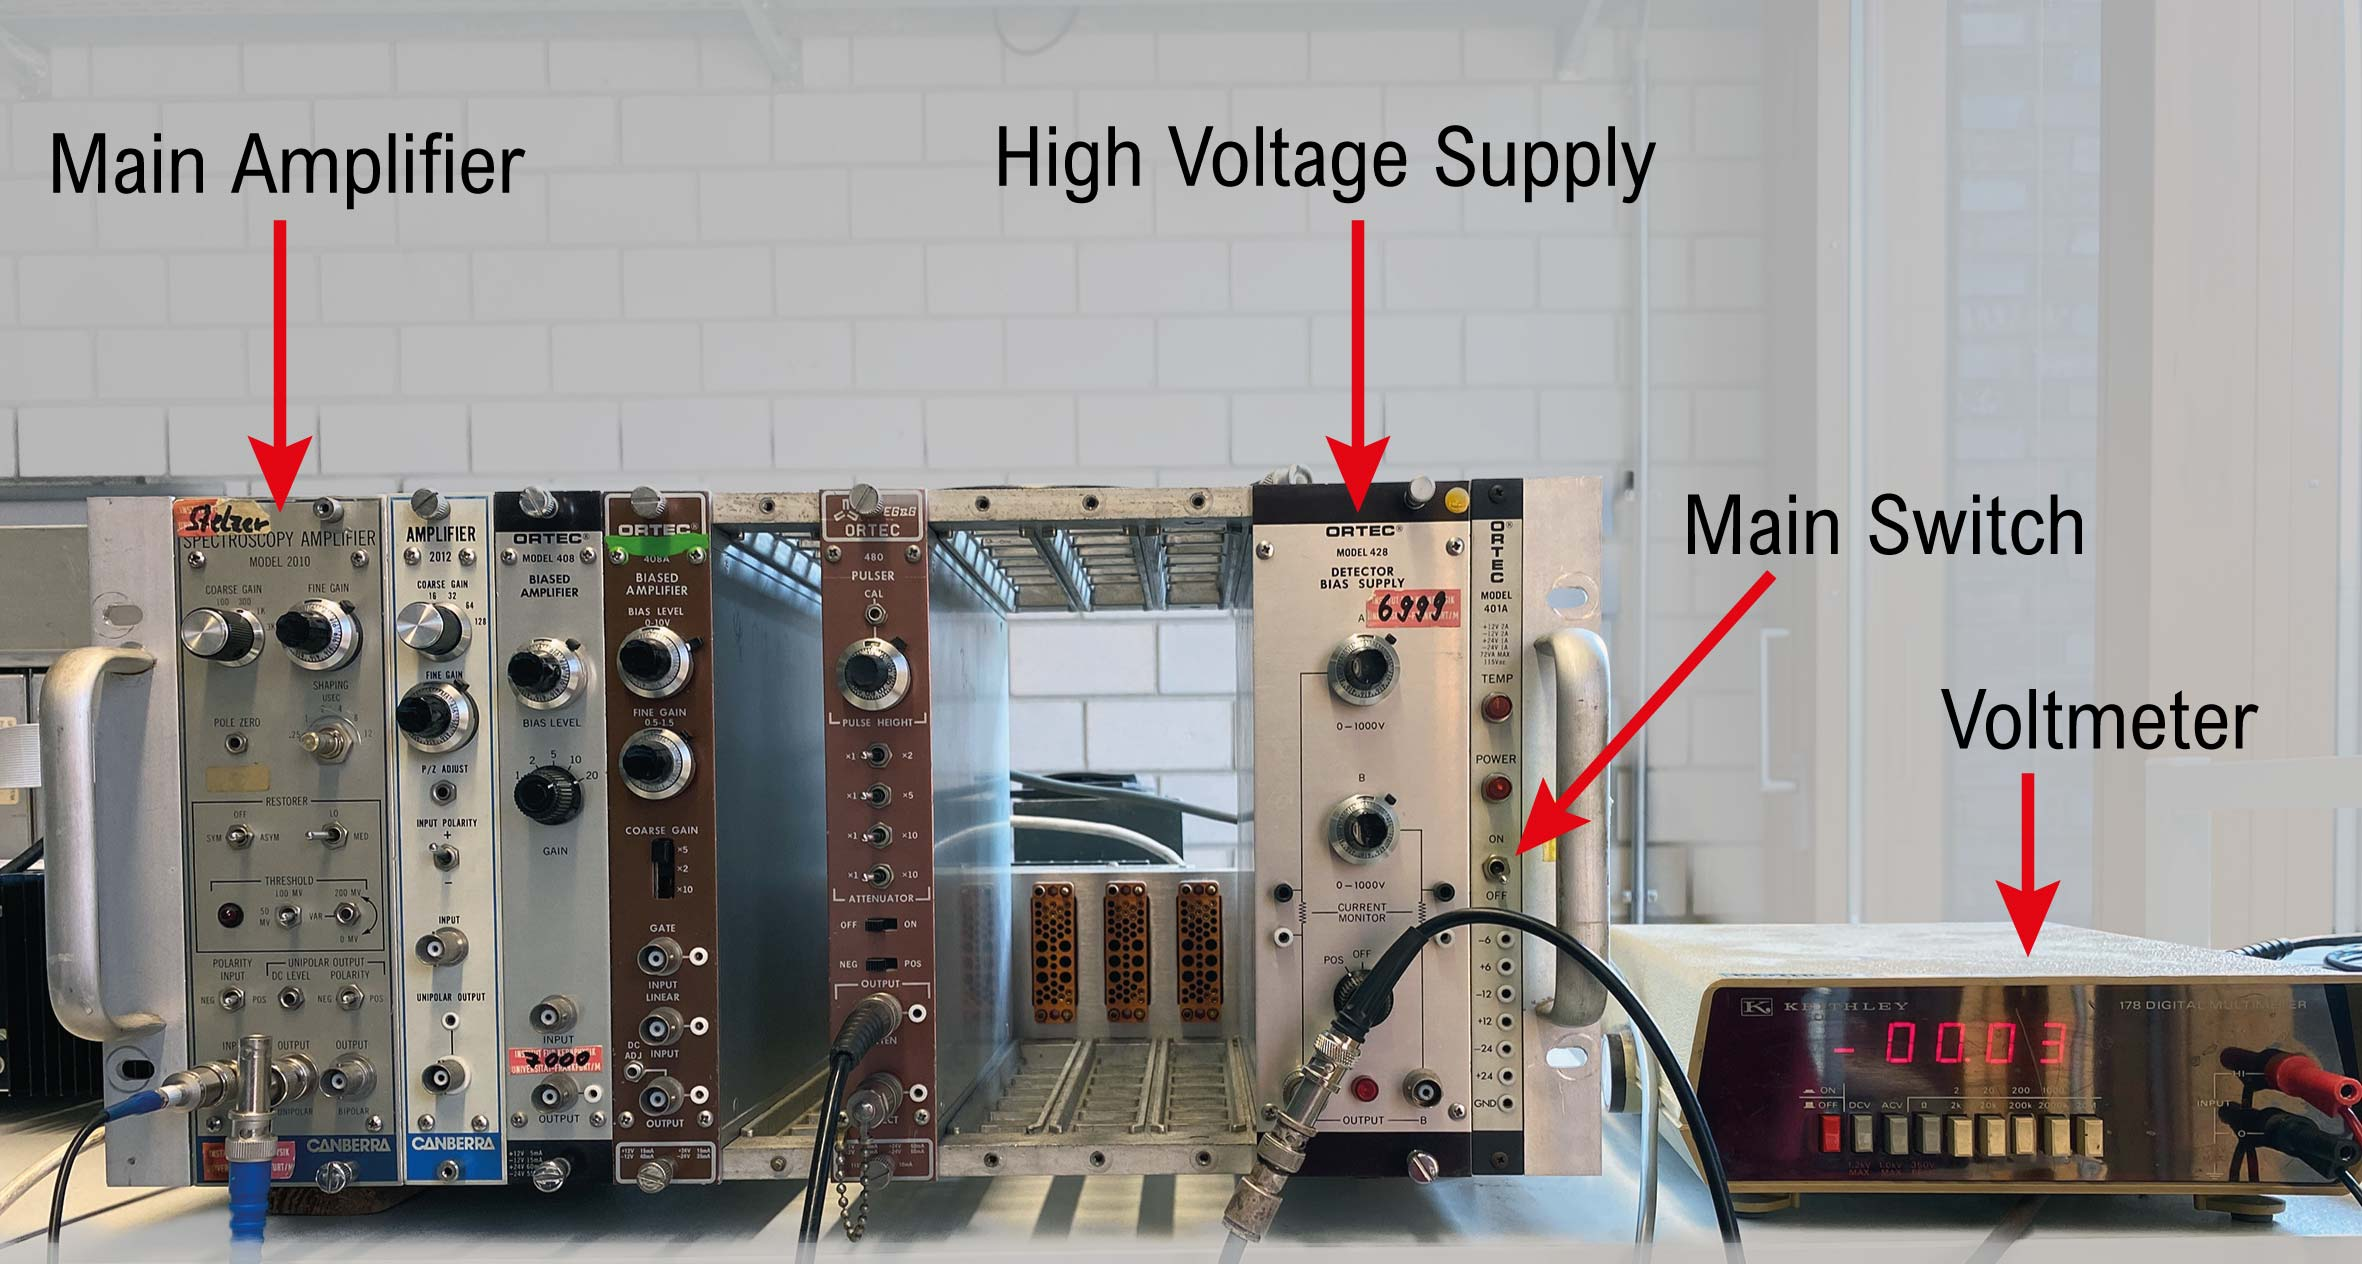
\includegraphics[width=0.75\linewidth]{img/setup_3.jpg}
	\caption{Zugehörige Elektronik im \enquote{Ortec-Crate}.}
	\label{fig:setup3}
\end{figure}



\clearpage
\section{Durchführung und Auswertung}
%
\subsection{Warnhinweise}\label{sec:warnhinweise}
%
\begin{minipage}[c]{.15\linewidth}
	
\includegraphics[width=1.5cm]{img/toxic}
\end{minipage}
\begin{minipage}[t]{.85\linewidth}
	Essen und Trinken ist im Labor untersagt.
\end{minipage}\vspace{1em}\\ 
\begin{minipage}[c]{.15\linewidth}
	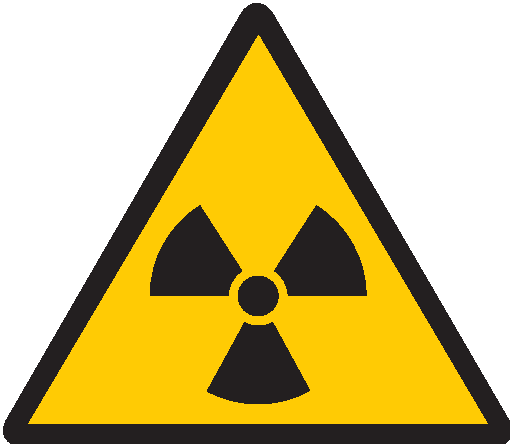
\includegraphics[width=1.5cm]{img/radioactive}
\end{minipage}
\begin{minipage}[t]{.85\linewidth}
	Die verwendete Strahlungsquelle sendet radioaktive Alphastrahlung aus. Sie ist schwach versiegelt und teilweise offen. Der Strahlenschutz sieht für solche Quellen besondere Sicherheitsmaßnahmen vor. Deshalb wurde das Präparat dauerhaft in der Apparatur installiert, sodass kein radioaktives Material aus der Apparatur in den Raum gelangen kann und kein Kontakt mit der Quelle möglich ist. Die Messapparatur darf deshalb auf keinen Fall geöffnet werden. Das Belüftungsventil soll so kurz wie möglich geöffnet bleiben.
\end{minipage}\vspace{1em}\\ 
\begin{minipage}[c]{.15\linewidth}
	
\includegraphics[width=1.5cm]{img/electric}
\end{minipage}
\begin{minipage}[t]{.85\linewidth}
	Die maximale Spannung am Halbleiterdetektor beträgt $200$ Volt. Die Spannung immer langsam verändern. Überschreiten der Spannung kann zur Zerstörung des Detektors führen.
	\\ \\
	Änderungen an der Verkabelung nur bei abgeschalteter Spannungsversorgung.
	\\ \\
	Der Detektor ist extrem lichtempfindlich, der Betrieb mit angelegter Hochspannung außerhalb der geschlossenen Vakuumkammer würde ihn zerstören.
\end{minipage}\vspace{1em}\\ 
\begin{minipage}[c]{.15\linewidth}
	
\includegraphics[width=1.5cm]{img/attention}
\end{minipage}
\begin{minipage}[t]{.85\linewidth}
	Be- und Entlüftungsventil des Vakuumkolbens nicht gleichzeitig öffnen.
	\\ \\
	Vor dem Be- oder Entlüften die Hochspannung abschalten. 
\end{minipage}\vspace{1em}\\ 
%
\clearpage
%
\subsection{Vorbereitungen}
Gehen Sie diese Checkliste gemeinsam mit dem/der Betreuer:in durch:
\begin{enumerate}
	\item Verkabelung kontrollieren (vgl. Abb. \ref{fig:verkabelung}).
	\item Sicherstellen, dass das Spannungsversorgungsgerät auf $0$ V eingestellt ist.
	\item Quelle auf kleinstmöglichen Abstand zum Detektor einstellen \\$r_{rel} = 0$ mm.
	\item Vakuumkammer evakuieren.
	\item Ortec-Crate einschalten.
	\item MCA3 Software auf dem PC starten.
\end{enumerate}

%
\subsection{Aufgabe 1: Sättigungsspannung}
Ziel der ersten Aufgabe ist die Bestimmung der Sättigungsspannung des Halbleiterdetektors. Die Messung erfolgt im Vakuum bei kleinstmöglichem Abstand $r_{rel} = 0$ mm.
\begin{enumerate}[label=\textbf{\alph*)}]
	\item Zeichnen Sie bei Detektorspannung $U_A = 0$ V ein Histogramm mit mindestens 8000 Counts auf. Bestimmen Sie 
		\begin{itemize}[nosep]
		\item die Peak-Position $\mu\ [\text{ADC Channels}]$,
		\item die Halbwertsbreite \textit{FWHM} [ADC Channels]
		\item und die Zählrate $Z$ [1/s]
	\end{itemize}
	des Plutonium-Peaks mithilfe eines Gauß-Fits in der Software.
	\item Wiederholen Sie a) für die Spannungen $U_A = 8, 15, 20, 25, 30, 40, 70, 100$ V
	\item Stellen Sie die Peak-Position $\mu$, die Zählrate $Z$ und die prozentuale Auflösung
		\begin{equation}
			d_E = \frac{\textit{FWHM}}{\mu} \cdot 100 \qquad [\%]
		\end{equation}
		in Abhängigkeit von $U_A$ grafisch dar.
	\item Bestimmen Sie ungefähr die Sättigungsspannung $U_{\text{sat.}}$ des Detektors anhand der Kurvenverläufe. Wählen Sie eine Spannung $U_{\text{Det.}}$ für Ihre folgenden Messungen. Erklären Sie Ihre Auswahl und die Bedeutung der Sättigungsspannung für die Benutzung des Halbleiterdetektors zum Energienachweis.
\end{enumerate}

\subsection{Aufgabe 2: Kalibrierung und Nullabstand}
Nun wird eine Energiekalibrierung des Multi-Channel-Analysators durchgeführt und der Null-Abstand $r_0$ zwischen Detektor und Quelle bestimmt. Die Messungen finden im Vakuum statt.

\begin{enumerate}[label=\textbf{\alph*)}]
	\item Stellen Sie die in Aufgabe 1 ermittelte Spannung $U_{\text{Det.}}$ an der Spannungsversorgung ein.
	\item Zeichnen Sie ein Referenzspektrum mit mindestens 12000 Counts bei $r_{rel} = 0$ mm auf.
		\\ Speichern Sie einen Screenshot des Referenzspektrums für Ihr Protokoll.
		\\ \textit{Optional:} Speichern Sie das Histogramm als \verb|.txt| Datei ab. Dies ermöglicht die Wiederholung der Kalibrierung zu Hause. 
	\item Kalibrieren Sie den Multi-Channel-Analyzer in der Software. \\Bestimmen Sie dazu die Position der drei Hauptmaxima im Histogramm per Gauß-Fit und verwenden Sie die passenden Austrittsenergien aus Abbildung \ref{fig:schemata}.
	
	Führen Sie die Gauß-Fits erneut durch, um die kalibrierten Werte für Positionen [keV] und Halbwertsbreiten [keV] sowie die Zählraten [1/s] zu erhalten.
	\item Zeichnen Sie bei den relativen Abständen $r_{rel} = 5, 10, 15, 20, 30$ mm jeweils mindestens 3000 Counts auf und bestimmen Sie auch hier per Gauß-Fit die kalibrierten Positionen, Halbwertsbreiten und Zählraten der drei Hauptmaxima.
	\item \textit{Am Versuchstag:} Stellen Sie die Zählrate in Abhängigkeit des relativen Abstandes für Plutonium grafisch dar.
	
	\textit{Im Protokoll:} Stellen Sie die Energie, die prozentuale Detektorauflösung und die Zählrate  jeweils in Abhängigkeit des relativen Abstandes für jedes der drei Isotope grafisch dar.
	\item Bestimmen Sie den Nullabstand $r_0$ zwischen Probe und Detektor, um bei den weiteren Messungen den effektiven Abstand $r_{eff} = r_0 + r_{rel}$ verwenden zu können. Überlegen Sie dazu, wie das Abstandsgesetz
	\begin{equation}
		Z \propto \frac{1}{r^2_{eff}}
	\end{equation}
	umgeformt und geschickt grafisch dargestellt werden kann, um den Nullabstand direkt vom y-Achsenabschnitt ablesen zu können. $Z$ ist hier die Zählrate $[1/s]$. Geben Sie auch das gemittelte Ergebnis aus den Messungen aller drei Isotope an.

    \textit{Anmerkung}: Betrachten Sie die Fehlerbalken und entscheiden Sie, ob Sie den Mittelwert oder den gewichteten Mittelwert mit varianzdefinierten Gewichten verwenden, um das Endergebnis $r_0$ zu erhalten. Letzteres ist definiert durch 

    \begin{subequations}\label{eq:weightmean}
    \begin{align}
		\overline{r_0} = \frac{\sum_i w_i r_{0,i}}{\sum_i w_i} \\
        \textnormal{mit Gewichten} w_i = \left( \Delta r_{0,i} \right)^{-2} \\\
        \textnormal{und Fehler } \Delta \overline{r_0} = \left( \sum_i w_i \right)^{-1/2}
    \end{align}
    \end{subequations}
\end{enumerate}

\subsection{Aufgabe 3: Reichweite in Luft}
Im letzten Teil des Versuches wird differenzielle Energieverlust der Alphastrahlung in Luft bestimmt.

\begin{enumerate}[label=\textbf{\alph*)}]
	\item Schließen Sie das Entlüftungsventil der Vakuumkammer. Öffnen Sie danach langsam das Belüftungsventil, bis der Atmosphärendruck in der Kammer hergestellt ist. Schließen Sie dann das Belüftungsventil wieder.
	\item Bestimmen Sie bei $r_{rel} = 0, 4, 8, 20, 24, 28, 32, 36, \dots$ mm mittels Gauß-Fit
	\begin{itemize}[nosep]
		\item die kalibrierte Peakposition $\mu\ [\text{keV}]$,
		\item die kalibrierte Halbwertsbreite \textit{FWHM} [keV]
		\item und die Zählrate $Z$ [1/s]
	\end{itemize}
	für die Hauptmaxima der drei Isotope. Erhöhen Sie den relativen Abstand weiter um je $4$ mm, bis das Plutoniumsignal bei $r_{max}$ verschwindet. Führen Sie dann noch drei zusätzliche Messungen bei $r_{rel} = r_{max} - 2, r_{max} - 6, r_{max} - 10$ mm durch. Zeichnen Sie für jede Messung mindestens 2000 Counts auf.
	\item \textit{Am Versuchstag:} Stellen Sie die $\alpha$-Energie $E\, \widehat{=}\, \mu$ abhängig vom effektiven Abstand für Plutonium grafisch dar.
	
	\textit{Im Protokoll:} Stellen Sie für alle drei Isotope die $\alpha$-Energie $E\, \widehat{=}\, \mu$, die prozentuale Auflösung und die Zählrate jeweils in Abhängigkeit vom effektiven Abstand grafisch dar.
	\item Bestimmen Sie näherungsweise -- durch Extrapolation mit dem Auge -- die Reichweite der $\alpha$-Teilchen und ihre Austrittsenergie anhand des Graphen, der effektiven Abstand gegen Energie zeigt. Wodurch wird die Unsicherheit der Ergebnisse am stärksten beeinflusst?
	
	Vergleichen Sie in einer Tabelle die Ergebnisse mit den Literaturwerten. Verwenden Sie dazu die angegebenen Austrittsenergien und das empirische Reichweitengesetz von Geiger, welches die Reichweite $R$ [mm] abhängig von der Austrittsenergie $E_0$ [MeV] der $\alpha$-Teilchen angibt:
	\begin{equation}\label{eq:geigerreachlaw}
		R = 3.1 \cdot \left(E_0\right)^{3/2}
	\end{equation}
	\textit{Optional:} Wenn Gleichung \ref{eq:geigerreachlaw} entsprechend umgeformt und angepasst wird, eignet sie sich als Fit-Funktion für die Daten. Damit können Reichweite und Austrittsenergie genauer als mit dem Auge bestimmt werden.
	\item \textit{Am Versuchstag:} Stellen Sie den differenziellen Energieverlust in Abhängigkeit des effektiven Abstands für Plutonium dar $\left( \Delta E/ \Delta x \ \text{vs.}\ r_{eff} \right)$.
	
	\textit{Im Protokoll:} Fügen Sie die Bragg-Kurven der anderen beiden Isotope hinzu. Schätzen Sie den Höchstwert des Energieverlusts und den Energieverlust in der Nähe der Probe. Vergleichen Sie die drei Kurven miteinander.
	\item Schätzen Sie die unterschiedlichen Beiträge ab, die in die Energieauflösung einfließen. Betrachten Sie die Detektorauflösung aus der Vakuum"= und der Luft"=Messung. Diskutieren Sie hierbei die Bedeutung des elektronischen Rauschens, der statistischen Schwankungen in der Anzahl der Elektronen"=Loch"=Paare (Fanofaktor), sowie die endliche Dicke des Strahler-Präparats und das Energiestraggeling.
\end{enumerate}
%
%
\subsection{Das Protokoll}
Reichen Sie zusammen mit dem Protokoll Ihre Original-Messdaten als ordentliche \texttt{.txt}-Datei ein, mit entsprechenden Kommentaren, um die Daten den jeweiligen Messungen zuordnen zu können. Der Aufbau des Protokolls sollte sich an den folgenden Punkten orientieren: 
%
\begin{itemize}
	\item Theorieteil
	\item Durchführung und Auswertung
	\begin{itemize}
		\item Was soll gemessen werden und warum?
		\item Welche Messergebnisse werden erwartet?
		\item Wie wird die Messung durchgeführt?
		\item Was wurde tatsächlich gemessen? Wie groß sind die Messfehler?
		\item Was kann aus dem Messergebnis gelernt werden? Wurden die Erwartungen erfüllt? Was sind die Fehlerquellen?
	\end{itemize}
	\item Fazit
\end{itemize}
%
\subsubsection*{Fehlerbehandlung}
Alle Daten in Ihren Diagrammen sollten sowohl mit x- als auch mit y-Fehlerbalken dargestellt werden.
Sie erhalten bei der Durchführung des Experimentes aus den Gauß-Fits bereits die Standardabweichungen zu den Messwerten. 
Für die übrigen Messwerte können Sie jeweils Annahmen zur Unsicherheit machen. 
Erstellen Sie Tabellen mit Messwerten und zugehörigen Unsicherheiten und weisen Sie die zur Berechnung verwendeten Formeln explizit aus.
Bei Größen, die aus mehreren (fehlerbehafteten) Messwerten ausgerechnet werden, führen Sie Gaußsche Fehlerfortpflanzung durch:
\begin{equation}\label{eq:RSS}
	\sigma_{f} = \sqrt{\left( \frac{\partial f}{\partial x_1}\ \sigma_{x_1} \right)^2 + \left( \frac{\partial f}{\partial x_2}\ \sigma_{x_2} \right)^2 + ... + \left( \frac{\partial f}{\partial x_n}\ \sigma_{x_n} \right)^2} 
\end{equation}
Hierbei errechnet sich die Messunsicherheit $\sigma_{f}$ von der Größe $f = f (x_1, x_2, ... , x_n)$, die abhängig ist von den Messwerten $x_1, x_2, ... , x_n$ und deren Unsicherheiten $\sigma_{x_1}, \sigma_{x_2}, ..., \sigma_{x_n}$. 






\newpage
\appendix
%
\section{Appendix}\label{sec:appendix}
%
\subsection{Your Report}
Together with the report, submit your original measurement data as a neat \texttt{.txt}-file with appropriate comments so that the data can be assigned to the respective measurements. The structure of the protocol should be based on the following points:
\begin{itemize}
	\item Theory section
	\item Execution and evaluation
	\begin{itemize}
		\item What is to be measured and why?
		\item What measurement results are expected?
		\item How is the measurement carried out?
		\item What was actually measured? How large are the measurement errors?
		\item What can be learned from the measurement result? Were the expectations met?
		What are the sources of error?
	\end{itemize}
	\item Conclusion
\end{itemize}
%
\subsubsection*{Error Handling}
All data in your diagrams should be displayed with both x and y error bars.
When carrying out the experiment, you will already receive the standard deviations for the measured values from the Gaussian fits. 
You can make sensible assumptions about the uncertainties of the other measured values. 
Create tables with measured values and associated uncertainties and explicitly state the formulas used for the calculation.
For variables that are calculated from several (error-prone) measured values, carry out Gaussian error propagation:
\begin{equation}\label{eq:RSS}
	\sigma_{f} = \sqrt{\left( \frac{\partial f}{\partial x_1}\ \sigma_{x_1} \right)^2 + \left( \frac{\partial f}{\partial x_2}\ \sigma_{x_2} \right)^2 + ... + \left( \frac{\partial f}{\partial x_n}\ \sigma_{x_n} \right)^2} 
\end{equation}
Here, $\sigma_{f}$ is the uncertainty of the quantity $f = f (x_1, x_2, ... , x_n)$, which is dependent of the measured values $x_1, x_2, ... , x_n$ and their respective uncertainties $\sigma_{x_1}, \sigma_{x_2}, ..., \sigma_{x_n}$. 

Alternatively, estimate the maximum error limits with
\begin{equation}\label{eq:abs}
		\sigma_{f} = \left| \frac{\partial f}{\partial x1}\right| \sigma_{x1} + \left| \frac{\partial f}{\partial x2}\right| \sigma_{x2} + ... + \left| \frac{\partial f}{\partial xn}\right| \sigma_{xn}
\end{equation}
%
\subsection{Notes}
%
\subsubsection*{Weighted Mean}
The weighted mean $\overline{x}$ of several measured values $x_i$ of the same quantity $x$ is defined as
\begin{subequations}\label{eq:weighted_mean}
    \begin{align}
    \overline{x} & = \frac{\sum\limits_{i}\ w_i \ x_{i}}{\sum\limits_{i} \ w_i }  \label{eq:wmean}\\
    \text{with weights } \quad w_i & = (\Delta x_{i})^{-2} \\
    \text{and error } \quad \Delta \overline{x} & = \left(  \sum\limits_{i} w_i  \right)^{-\frac{1}{2}} \label{eq:wmeanerr}
    \end{align}
\end{subequations}
here, $\Delta x_i$ is the uncertainty of the $i$-th single measurement value.


\clearpage
\begin{thebibliography}{1}
	\bibitem{kolanoski} 
	Kolanoski, H., Wermes, N., 2016. \emph{Teilchendetektoren}. Springer-Verlag Berlin Heidelberg. \textsc{doi:} \url{https://doi.org/10.1007/978-3-662-45350-6}
	
	\bibitem{povh-rith}
	Povh, B., Rith, K. u.a., 2014. \emph{Teilchen und Kerne}. Springer-Verlag Berlin Heidelberg. \textsc{doi:} \url{https://doi.org/10.1007/978-3-642-37822-5}
	
	\bibitem{leo}
	Leo, W.R., 1994. \emph{Techniques for Nuclear and Particle Physics Experiments: A How-To Approach}. Springer Berlin / Heidelberg. ISBN 9783642579202. 
	
	\bibitem{pdg}
	Particle Data Group, Workman, R. L. u.a., 2022, \emph{Review of Particle Physics}, \textsc{in:} Progress of Theoretical and Experimental Physics 2022, Issue 8, 083C01, \textsc{doi:} \url{https://doi.org/10.1093/ptep/ptac097}
	
	\bibitem{NDS2014} % Quelle für Energien von Plutonium
	Browne, E., Tuli, J.K. 2014. Nuclear Data Sheets 122, 205 (2014). \url{https://www.nndc.bnl.gov/nudat3/decaysearchdirect.jsp?nuc=239Pu&unc=NDS}
	
	\bibitem{NDS2006} % Quelle für Energien von Americium
	Basunia, M.S., 2006. Nuclear Data Sheets 107, 3323 (2006). \url{https://www.nndc.bnl.gov/nudat3/decaysearchdirect.jsp?nuc=241Am&unc=NDS}
	
	\bibitem{NDS2008} % Quelle für Energien von Curium
	Singh, B., Browne, E., 2008. Nuclear Data Sheets 109, 2439 (2008). \url{https://www.nndc.bnl.gov/nudat3/decaysearchdirect.jsp?nuc=244Cm&unc=NDS}

	\bibitem{bleck-neuhaus}
	Bleck-Neuhaus, J., 2013. \emph{Elementare Teilchen: Von den Atomen über das Standard-Modell bis zum Higgs-Boson}. Springer-Verlag Berlin Heidelberg. 2. Aufl. \textsc{doi:} \url{https://doi.org/10.1007/978-3-642-32579-3}
	
	\bibitem{dewiki:240085809}
	Wikipedia, 2023, \emph{Alphastrahlung}, \url{https://de.wikipedia.org/w/index.php?title=Alphastrahlung&oldid=240085809},
	[Online; Stand 5. März 2024]
	
	\bibitem{img:coulombwall}
	Johannes Schneider, CC BY-SA 4.0, \url{ https://commons.wikimedia.org/w/index.php?curid=61182444}
\end{thebibliography}


	
\end{document}